%%
%% This is file `thesis.tex',
%% generated with the docstrip utility.
%%
%% The original source files were:
%%
%% scnuthesis.dtx  (with options: `thesis')
%%
%% !Mode:: "TeX:UTF-8"
%%
%% This is a generated file.
%%
%% Copyright (C) 2015 by Joseph Pan <cs.wzpan@gmail.com>
%%
%% This file may be distributed and/or modified under the
%% conditions of the LaTeX Project Public License, either version 1.3a
%% of this license or (at your option) any later version.
%% The latest version of this license is in:
%%
%% http://www.latex-project.org/lppl.txt
%%
%% and version 1.3a or later is part of all distributions of LaTeX
%% version 2004/10/01 or later.
%%
%% To produce the documentation run the original source files ending with `.dtx'
%% through LaTeX.
%%
%% Any Suggestions : Joseph Pan <cs.wzpan@gmail.com>
%% Thanks LiuBenYuan <liubenyuan@gmail.com> for the nudtpapre class!
%% Thanks Xue Ruini <xueruini@gmail.com> for the thuthesis class!
%% Thanks sofoot for the original NUDT paper class!
%%
%1. 如果是研究生论文,常用的选项是:
% \documentclass[master,twoside,vista,ttf]{scnuthesis}
%2. 如果是博士生论文,常用的选项是:
% \documentclass[doctor,twoside,vista,ttf]{scnuthesis}
%3. 如果使用是Windows XP之前的Windows系列,或者使用从这个系列拷贝过来的字体,则需要将Vista选项去掉,如:
% \documentclass[master,twoside,ttf]{scnuthesis}
%4. 建议使用OTF字体获得较好的页面显示效果
%   OTF字体从网上获得,各个系统名称统一,不用加vista选项
%   如果你下载的是最新的(1201)OTF英文字体,建议修改scnuthesis.cls,使用PS Std
%   \documentclass[doctor,twoside,otf]{scnuthesis}
%5. 如果想生成盲评,传递anon即可,仍需修改个人成果部分
% \documentclass[master,otf,anon]{scnuthesis}
%6. 让章节标题作为页眉,可以使用chapterhead选项。如果和twoside 一起使用,则奇数页页眉为章节标题,偶数页为文章标题。
% \documentclass[master,otf,twoside,chapterhead]{scnuthesis}
%
\documentclass[master,vista,ttf,twoside]{scnuthesis}
\usepackage{myscnu}

\begin{document}
\graphicspath{{figures/}}


\classification{}  % 分类号
\udc{}             % UDC号
\mastertype{学术}  % 硕士学位类型(只用于硕士论文)
\confidentiality{公开}  % 密级
\serialno{2016022292}
\title{基于时序和迁移学习的神经网络推荐算法研究}
\entitle{Research on transfer learning and sequential in recommendation}
\displaytitle{基于时序和迁移学习的神经网络推荐算法研究}
\author{付海林}
\enauthor{Hailin Fu}
\subject{软件工程}
\ensubject{Software Engineering}
\researchfield{数据挖掘}
\school{计算机学院}
\supervisor{李建国}
\ensupervisor{Jianguo Li}
\protitle{}
\zhdate{\zhtoday}

% 插入摘要,制作封面
\ifisanon{}
\else{\maketitle}
\fi

\frontmatter

\begin{cabstract}
互联网技术迅速发展,各行各业的数据都在指数膨胀,科研领域也一样,数据量急速的增长给科研人员带来%
了丰富的信息,同时也带来了许多难题。作为科研学者,需要实时保持追踪学术的新动态,然而,通过人工%
从海量数据中筛选出与自己研究领域相符的学者,无疑是一个非常浩大的工程。因此,本文使用自然语言处%
理方面的技术快速提取文本的关键词,再结合图论相关算法,快速筛选出与用户学者研究兴趣相符的科研学者,%
进而推荐给学者用户,以帮助科研人员节省时间,减小工作量。%

本文提出了一个基于关键词的学者推荐模型,该模型包含挖掘论文学者研究领域(关键词提取)、用户学者兴趣%
(关键词网络)和打分推荐三个子模块。主要流程是通过融合多种特征从论文摘要中提取出关键词集合,将关键%
词集作为论文学者研究领域;接着,将关键词集和用户学者搜索的关键词结合,构建以共现为关系的词图KOG,%
通过多种算法挖掘KOG图得到该图的核心节点,本文将得到的核心节点作为对用户学者偏好或者兴趣的一个扩展;%
最后,构建论文作者(Author)-关键词(Keyword)的二部图AKG,来对论文学者用户打分排序,%
其中关键词出现在论文学者的摘要中,作者节点和关键词节点之间就存在边相连。本文充分利用关键词%
去挖掘用户学者-论文学者之间的隐式联系。%

本文之所以关键词作为切入点,是因为短小精悍的关键词不仅能够代表一篇论文的主题,而且其本身%
蕴含着丰富的信息,其被广泛的应用在文本分类、聚类、搜索、推荐等领域。本文只考虑使用关键词%
(不使用任何其它的特征,例如论文引用数、作者影响力、用户学者的基本信息或者历史记录等)实%
现学者推荐,所以本文对于解决推荐系统中的冷启动问题有很重要的作用。无论是从用户学者的角度还是%
从论文学者的角度考虑,本模型都围绕关键词展开,关键词是影响该学者推荐模型准确率的唯一因素,%
因此,关键词抽取问题即是本文研究的核心部分,本文提出了融合多特征的关键词抽取算法,并对结果进行评估。%

本文在KDD、WWW真实的论文数据集进行关键词提取的对比实验。为了验证本文推荐框架的有效性,%
本文爬取了Microsoft
Academic官网的生物医学论文数据进行实验验证,实验证明,该推荐模型到不错的准确率,%
能进行有效的推荐,对于解决大数据时代信息过载问题,本文的研究具有重要的实际意义。

\end{cabstract}
\ckeywords{学者推荐;关键词抽取;词网络挖掘;核心点选取;冷启动}

\begin{eabstract}
  
\end{eabstract}
\ekeywords{scholar recommendation; extract keyword; cold start }




% 生成目录
\tableofcontents

\renewcommand{\chapterlabel}{\denotationname} % 设置页眉


% 书写正文,可以根据需要增添章节。
\mainmatter
%!TEX root = ../document.tex
\chapter{绪论}
\section{研究背景与意义}

我国经过二十余年的信息化建设,互联网用户仍在持续增长,根据中国互联网信息中心发布的第43次《中国互联网络发展%
状况统计报告》\upcite{43CNNIC}显示,截止2018年12月,我国网民规模达8.29亿,较2017年末仍增加了3.8\%,互联%
网普及率达59.6\%,其中移动互联网用户比例更是高达98.6\%。
浩如烟海的数据填充着互联网,人们要从海量数据中找到自己关心的部分变得越来越难。
推荐系统是帮助用户从海量产品集合里面找到感兴趣目标的软件应用,具有千人千面的特点,也是数据挖掘和机器学习%
相关科技在实践领域最成功的应用之一。
在许多网站和应用程序中,例如电子商务、新闻和视频网站、%
音乐和广播电台等,他们都需要为用户推荐可能喜欢物品的杰出服务,如今接收不同形式的自动推荐已经成为我们日常%
在线用户体验的一部分。在典型的在线网站上面,可以收集用户各种类型的相关动作,例如:用户点击、浏览、收藏、购买%
了某个商品。
推荐系统(RS)已发展成为帮助用户做出明智决策和选择的基本工具,尤其是在大数据时代,%
客户必须从大量产品和服务中做出选择。因此现代推荐系统是在当前大数据环境下应运而生的,%
现代推荐系统的架构如图\ref{fig:RS_Architecture}所示,本文讨论的问题主要出于推荐算法层面。

\begin{figure}[htb]
  \centering
  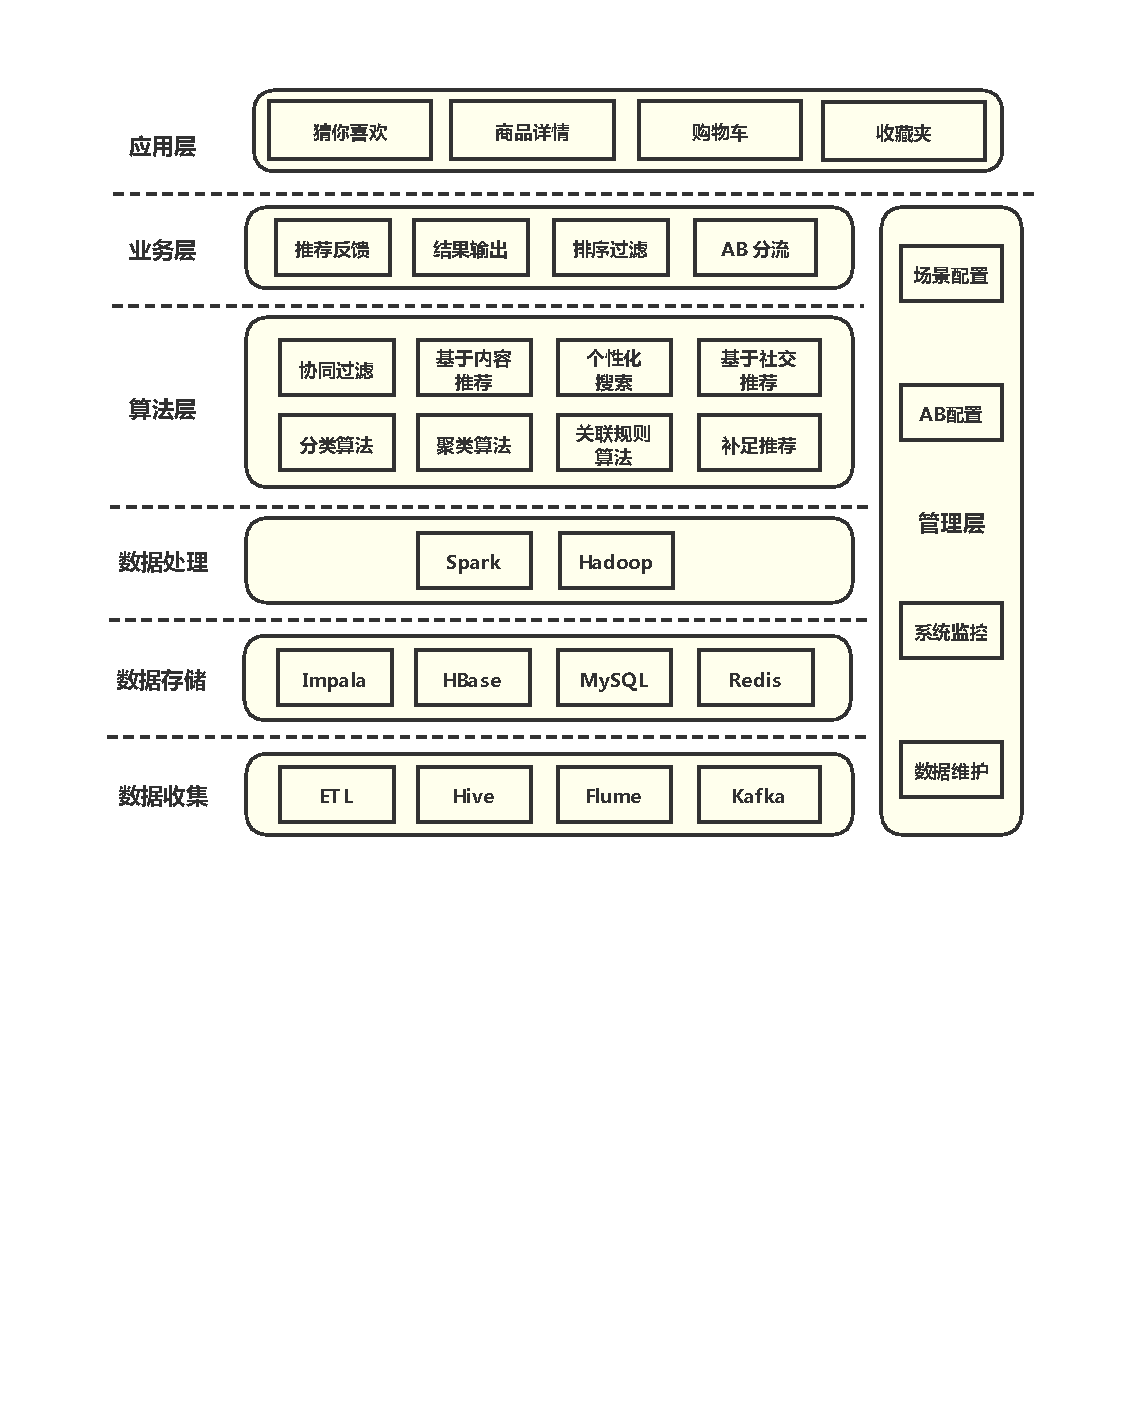
\includegraphics[width=\linewidth]{RS_Architecture.pdf}\\
  \caption{现代推荐系统架构图}
  \label{fig:RS_Architecture}
\end{figure}
推荐算法作为推荐系统的灵魂,承担着推荐高品质项目和高效反馈的重任,因此设计鲁棒性好的推荐算法有着重要的研究意义。
现有的推荐策略都主要关注如何为用户或项目找到临近集,或者利用其它的显式或隐式信息(如标签、评论、%
项目属性和用户个人信息)来提升近邻感知能力。然而,这些静态算法都没有考虑用户兴趣变化的实时动态性。时序信息%
就是反应用户兴趣实时变化的一个重要特征,在许多任务比如用户下一行为预测中,用户下一首会听什么歌与用户的%
喜好、当前所处环境的上下文都高度相关。

推荐系统面对的任务主要有两部分:评分预测和产品推荐。所以根据用户的历史%
记录预测他下一次会选择什么也是推荐领域一个严峻的挑战。

% 推荐系统面临的另外一个巨大挑战就是处理新用户和新物品,也就是所谓的冷启动问题,因为这些用户/物品的特征在缺少数据时很难正确判断。近来,迁移学习\upcite{YangTransfer}被用于解决推荐系统的冷启动问题。迁移学习通过利用辅助域来在目标域上获得提升


因此本文提出序列建模的推荐思路,本文的研究内容是结合神经网络的序列建模技术和推荐系统相关理论知识,实现快速向用户推荐可能感兴趣的物品。%
充分利用深度神经网络强大的建模能力,提取用户行为的重要时序特征,构建推荐对象的兴趣模型,%
% 再结合迁移学习的泛化能力,
构建相关模型来识别用户的兴趣意图,综合考虑推荐对象和用户两者之间%
的特征信息挖掘两者之间的隐式联系,从而发掘出用户感兴趣的物品,
以此来帮助用户快速的找到有感兴趣的物品,提升网络应用的流量及用户的黏性。%






%
本章节主要从传统机器学习和深度学习两个方面介绍现代推荐系统中常用的各种推荐算法,%
从它们各自的特点分析现如今存在的问题。

\section{国内外研究现状}

为了分析和理解国内外现有推荐算法的各自特点,本章节根据其使用的技术不同分为两个大类分别进行描述,
同时给出了如图\ref{fig:RA_clsssification}的思维导图。

\begin{figure}[htb]
  \centering
  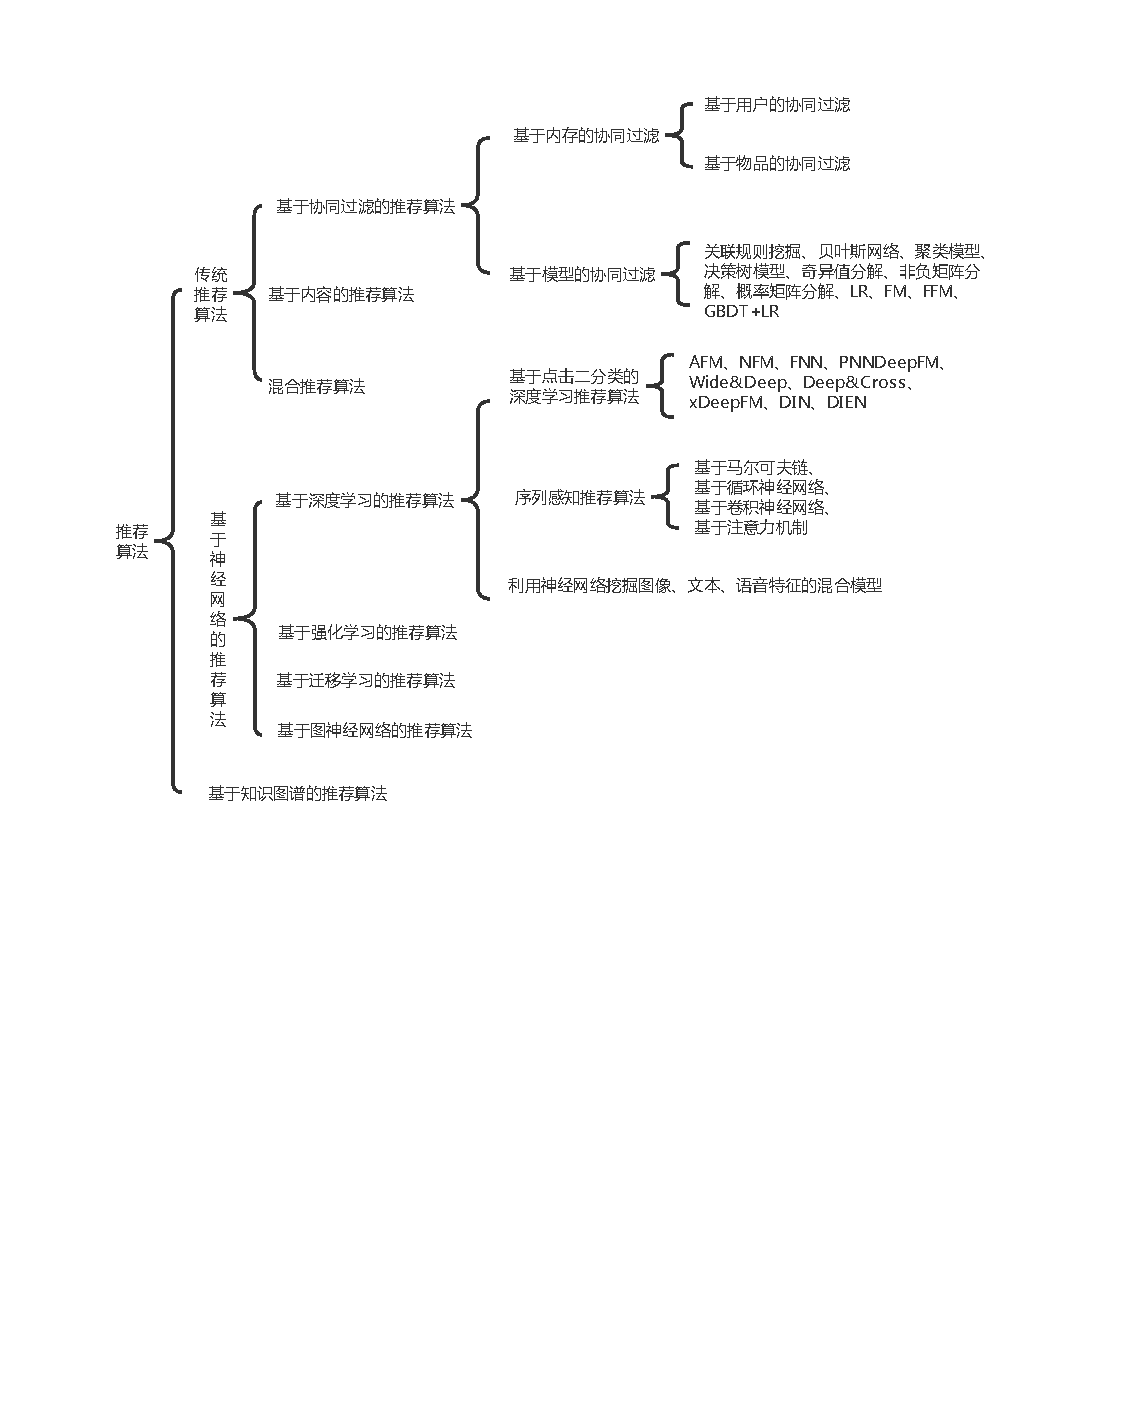
\includegraphics[width=\linewidth]{RA_clsssification.pdf}\\
  \caption{推荐算法分类思维导图}
  \label{fig:RA_clsssification}
\end{figure}

\subsection{传统推荐算法}

传统的经典推荐算法主要可分为三大类,它们分别是基于协同过滤的推荐算法、基于内容的%
推荐算法和混合推荐算法。协同过滤算法大体上可以分为基于内存的协同过滤(Memory-based CF)%
和基于模型的协同过滤(Model-based CF)。基于内存的协同过滤通过为用户寻找具有相似行为的用户%
或有相似特点的物品集合做推荐,所以可细分为基于用户的协同过滤%
(User-based Collaborative Filtering,UBCF)和基于物品的协同过滤%
(Item-based Collaborative Filtering,IBCF)。
而基于模型的协同过滤则主要利用评分信息训练相应的模型,然后使用这个模型对未知数据进行预测,%
这类算法有贝叶斯网络\upcite{Chen02abayesian}、聚类模型\upcite{ungar1998clustering}、%
概率矩阵分解\upcite{Salakhutdinov:2007:PMF:2981562.2981720}等等。
在基于内容的推荐算法中仅利用了单个用户的行为和数据给出对用户的推荐,特别是物品的描述和用户的属性描述在内容推荐中起到了关键作用。基于内容的
推荐精确度往往有限,还面临着严重的冷启动问题。
混合推荐系统则通过将上述两大类算法中的一个或多个结合起来以避免和克服某个单一算法带来的缺点。混合推荐算法中比较常见的方式是将基于内容的推荐方法与其他方法进行融合以避免冷启动、数据稀疏和扩展性等问题。
基于传统推荐算法的特点,%
基于协同过滤的推荐算法中大多需要构造一个用户与物品的交互矩阵,随着大数据的极速发展,%
物品与用户的数量往往能达到上亿规模,使得交互矩阵构造的空间复杂度过高,在大数据时代传统推荐算法已慢慢无法解决当%
前所面对的问题。

\subsection{基于深度学习的推荐算法}

得益于神经网络的反向传播理论,批量梯度下降的网络权重优化方式使得机器学习特别是深度学习%
能处理的数据规模没有理论上的数量限制,现代推荐算法也借助神经网络的技术蓬勃发展。%
神经网络领域下面子领域里的许多技术都已经被应用于推荐系统当中,包括深度学习、强化学习、迁移学习和图神经网络。%
本文仅讨论基于深度学习的推荐算法。

学术界推荐算法的发展离不开工业界的实践,而推荐算法在工业界的实践应用也为学术界的发展指引着方向。
推荐算法在工业界的一个重要实践就是进行点击率预估。随着深度学习技术被引入点击率预估方面,开始有大量的成果诞生。
点击率预估的通常做法是将推荐问题转化为二分类的有监督学习问题,算法建模的样本对象是物品,将用户的特征与物品特征拼接在一起构造高维样本,预测对象用户是否可能会点击目标物品。
在深度学习技术没有被引入点击率预估之前,传统做法通常使用逻辑回归\upcite{Kondakindi2014ALR}进行点击二分类,但这需要构造大量手工特征,FM\upcite{Rendle:2010:FM:1933307.1934620,Rendle:2012:FML:2168752.2168771}、FFM\upcite{Juan:2016:FFM:2959100.2959134}和GBDT+LR\upcite{He:2014:PLP:2648584.2648589}的出现让这类点击二分类模型能够自动学习到一些二维组合特征或者一些高维特征。随着深度学习的引入,特征的挖掘变得更加充分,组合特征的学习变得更加高效。

深层神经网络模型引入到点击二分类算法当中大多是通过神经网络与其他基础算法结合的方式构建混合模型,这些方法根据其网络融合的方式大致可以分为\textbf{串行融合}和\textbf{并行融合}两大部分。
\textbf{串行融合}的方式主要将FM等模型的输出作为MLP的输入,将FM视为交叉特征提取器,这类模型有:
Weinan Zhang等在 2016 年提出的因子分解机神经网络(Factorisation Machine supported Neural Network,FNN)\upcite{Zhang_2016},其将考FM与MLP进行了串联结合,利用FM为多层感知机MLP提取二维交叉特征进行点击率预估推荐;
Xiangnan He等在2017 年提出的神经网络因子分解机(Neural Factorization Machines,NFM)\upcite{He_2017}加入了池化层,将FM生成的二维交叉特征进行了元素级别的两两向量内积,引入了更多的非线性关系;
和Jun Xiao等人在2017年提出了注意力因子分解模型(Attentional Factorization Machine,AFM)\upcite{Xiao_2017},用注意力网络替换了上述两个模型中MLP,让Attention网络更好利用FM的二阶特征;Yanru Qu等人在2016年提出了基于向量积的神经网络(Product-based Neural Networks,PNN)\upcite{Qu_2016},与NFM不同的是使用了FM生成的二维交叉特征进行了元素级别的两两向量内积进行计算。
\begin{figure}[htb]
  \centering
  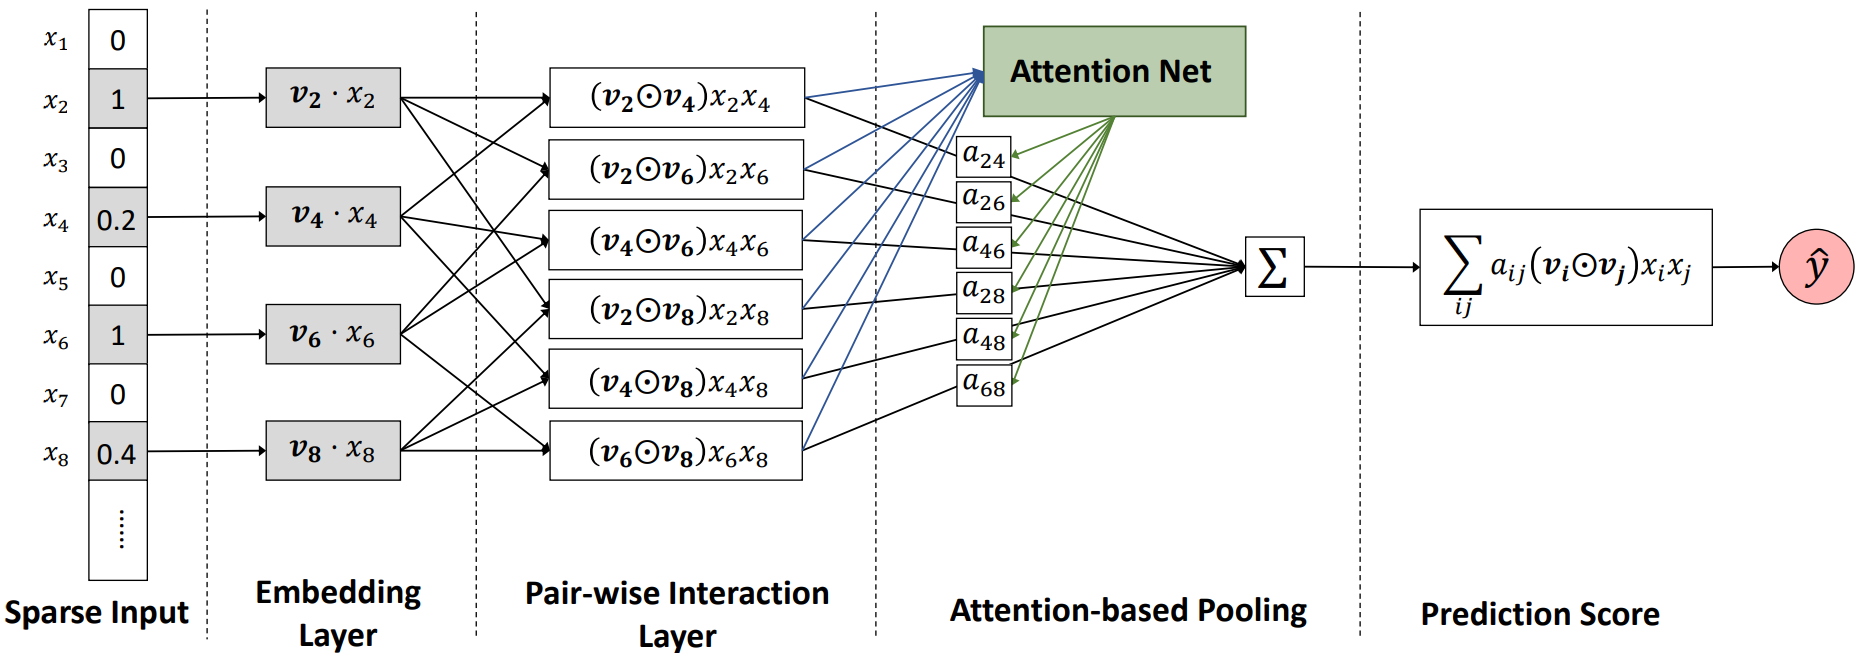
\includegraphics[width=\linewidth]{AFM.png}\\
  \caption{串行深度网络推荐模型之——AFM网络结构图\upcite{Xiao_2017}}
  \label{fig:AFM}
\end{figure}

而\textbf{并行融合}的方式则是利用两个或多个网络模块,每个子模块负责提取不同维度的特征为主要思路,构建点击二分类算法。这类模型主要有:


2017年Huifeng Guo等人将FM与MLP并行连接,提出的DeepFM模型\upcite{ijcai2017-239},两个组件网络共享同一个输入并行训练,能同时提取特征的低维和高维特征;
2016年Heng-Tze Cheng等人将一个Wide网络模型与深层网络Deep模型并行连接,利用Wide模块提升模型的记忆性,利用Deep模块提升模型的泛化性,构造的Wide\&Deep模型\upcite{Cheng_2016};
2017年Ruoxi Wang等人将深层网络Deep与一个交叉网络Cross并行连接,利用不同层数的Cross网络构造出任意维度的交叉特征,提出了Deep\&Cross模型\upcite{Wang:2017:DCN:3124749.3124754};
2018年Jianxun Lian等人提出了一个新颖的压缩交互网络(Compressed Interaction Network, CIN)的神经模型用于自动学习显式的高阶特征交互,然后将其与DNN模块并行集成,构造了一个名为极深因子分解机的模型(xDeepFM)\upcite{Lian:2018:XCE:3219819.3220023}用于同时以显式和隐式的方式自动学习高阶的特征交互。
\begin{figure}[htb]
  \centering
  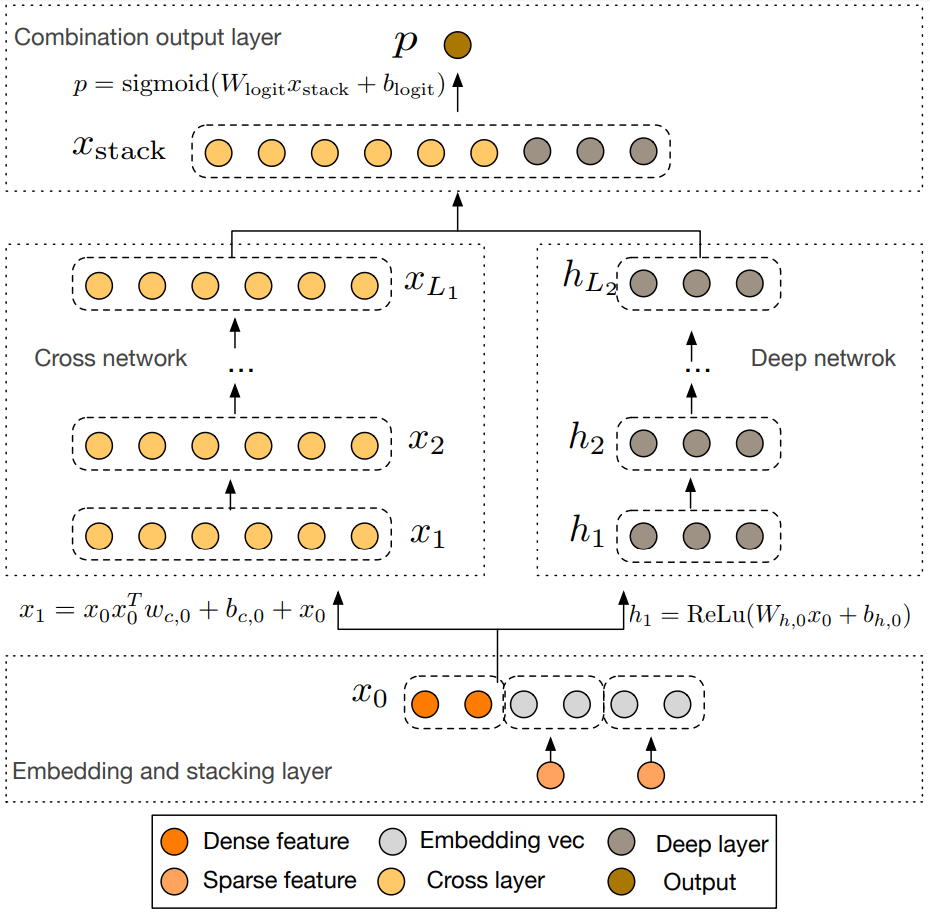
\includegraphics[width=\linewidth]{Deep_Cross.png}\\
  \caption{并行深度网络推荐模型之——Deep\&Cross网络结构图\upcite{Wang:2017:DCN:3124749.3124754}}
  \label{fig:Deep_Cross}
\end{figure}

在串行模型与并行模型之外,又有一类\textbf{综合并行结构与串行的结构},如2018年Guorui Zhou等人先后提出了深度兴趣网络(Deep Interest Network,DIN)\upcite{Zhou:2018:DIN:3219819.3219823}和深度兴趣演化网络(Deep Interest Evolution Network ,DIEN)\upcite{zhou2018deep},DIN的并行结构体现在对用户侧历史行为特征域和物品侧特征域并行嵌入,堆叠组合成的向量再输入到全连接神经网络中去。DIEN对DIN的改进在于并行结构的特征嵌入部分考虑到了用户兴趣的演化进程,其使用双层GRU对用户历史行为的序列进行建模,将建模后的向量一起并入堆叠向量当中。

\subsection{序列感知推荐研究现状}

现有的推荐算法几乎很少有考虑到隐藏在用户历史行为序列中的用户兴趣动态变化情况,而且以上提到的基于深度学习的推荐算法都是以构造大量特征为基础进行建模的,这些算法都需要收集大量用户隐私数据,况且在某些特殊应用场景下,例如用户在使用在线服务但并未登陆或匿名的情况下,以构造大量特征为前提的算法将全部失效。考虑到这三类情况,本文提出了序列感知推荐算法,以用户历史行为组成的序列为数据进行建模推荐,无需使用大量用户隐私相关数据,在用户匿名状态下也可以根据当前服务的会话构成行为序列。
序列感知推荐算法许多学者称为基于会话的推荐算法,其中使用的序列建模算法基本可以分为RNN和CNN两大方向。在使用RNN进行序列建模推荐算法中,其中最广为人知的工作为2016年Balazs Hidasi等于提出的使用循环神经网络的基于会话的推荐算法GRU4Rec\upcite{DBLP:journals/corr/HidasiKBT15},首次通过使用循环神经网络利用会话的序列进行建模推荐,这类使用循环神经网络对序列进行建模进行推荐的还有Devooght等人于2017年提出的\upcite{devooght2016collaborative,Devooght:2017:LSR:3079628.3079670},2017年Yu Zhu等人在使用LSTM对序列建模的基础上加上了对时间间隔的考虑,提出了Time-LSTM模型\upcite{ijcai2017-504}。
\begin{figure}[htb]
  \centering
  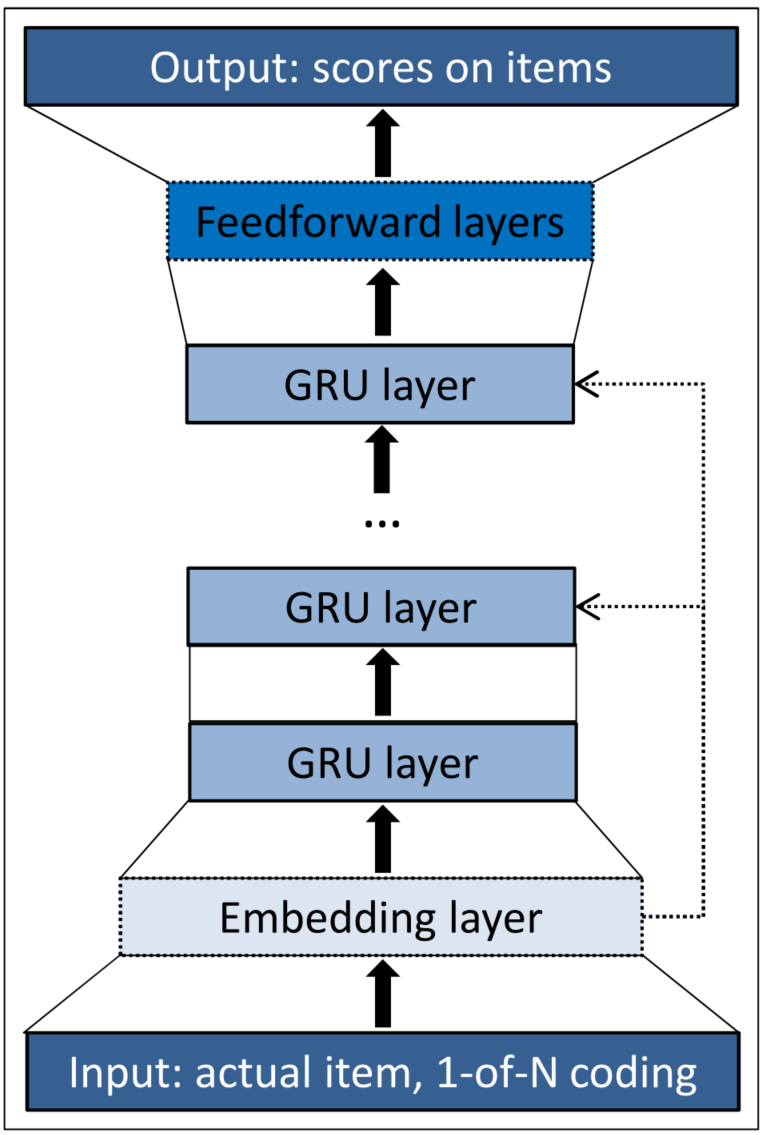
\includegraphics[height=6cm]{GRU4Rec.png}\\
  \caption{使用循环神经网络进行序列推荐算法之——GRU4Rec网络结构图\upcite{DBLP:journals/corr/HidasiKBT15}}
  \label{fig:GRU4Rec}
\end{figure}
基于RNN的序列建模方法有较好的性能,但受固于RNN的递归结构,算法难以并行实现。

另外一类序列感知推荐算法的方向是使用CNN对用户行为历史记录进行序列建模,CNN常用于计算机视觉领域图像特征提取,用于序列建模需要对基本的卷积结构进行大量的修改,这其中知名的工作有2018年Jiaxi Tang等人将序列嵌入矩阵使用CNN提取特征,提出的卷积序列嵌入推荐模型Caser\upcite{Tang:2018:PTS:3159652.3159656}。
\begin{figure}[htb]
  \centering
  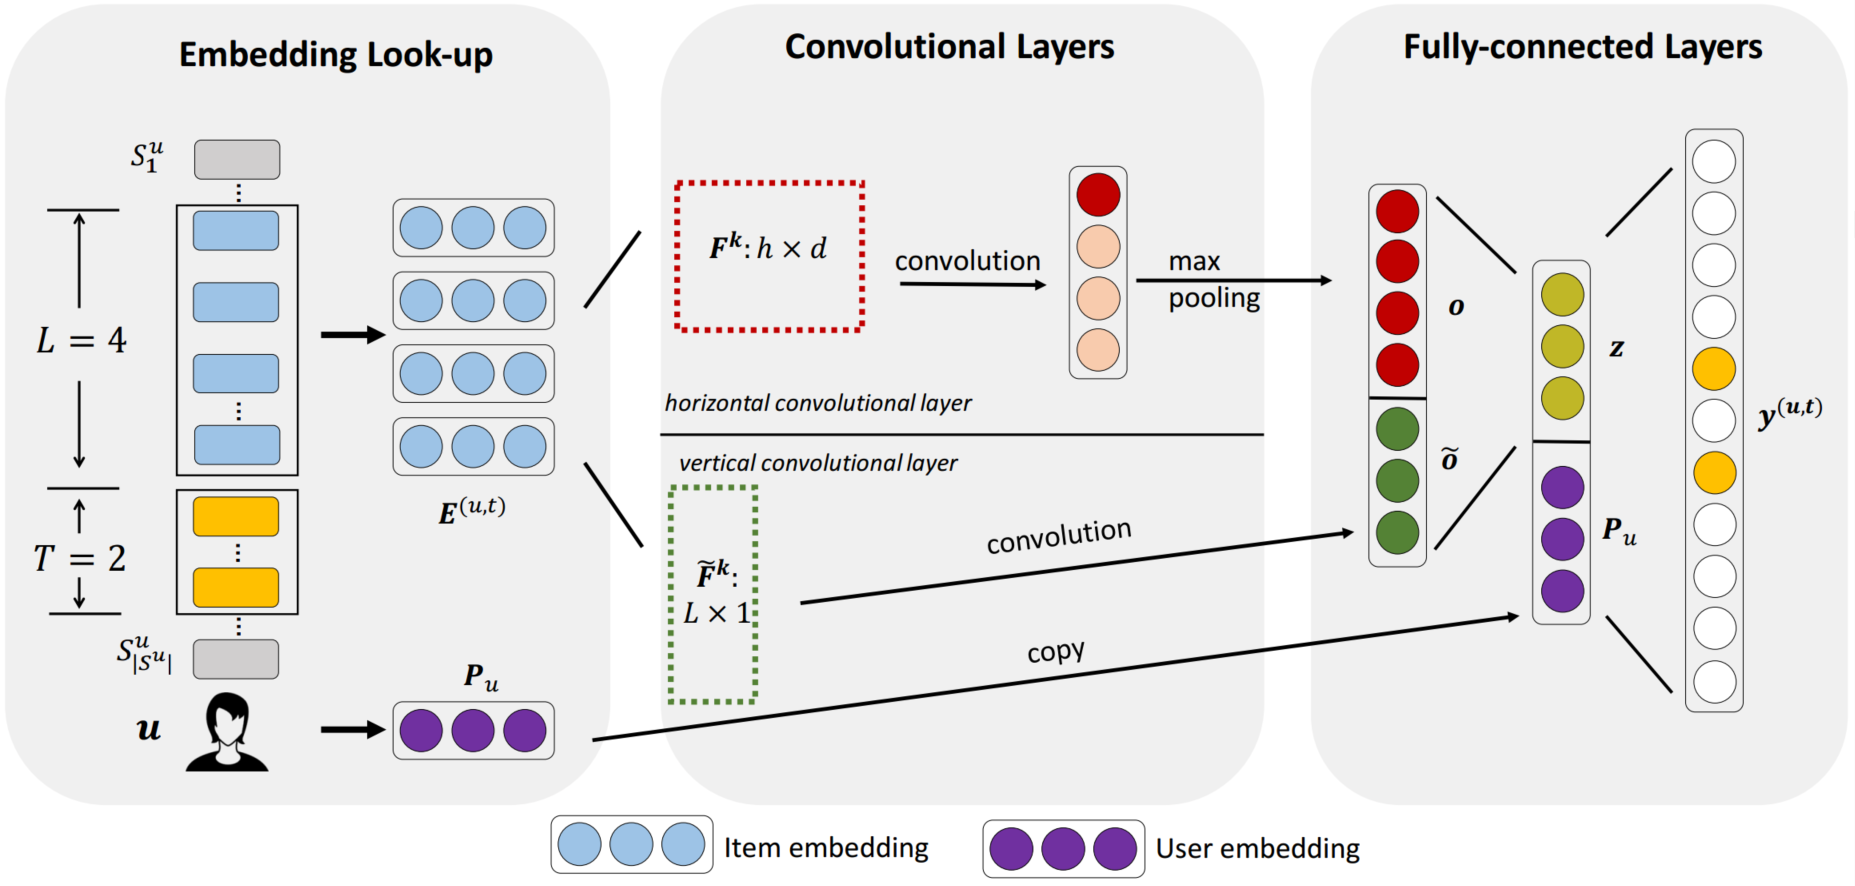
\includegraphics[width=\linewidth]{Caser.png}\\
  \caption{使用卷积神经网络进行序列推荐算法之——Caser网络结构图\upcite{Tang:2018:PTS:3159652.3159656}}
  \label{fig:Caser}
\end{figure}
基于CNN的序列建模方法记忆的序列长度严重依赖卷积层的深度。

\section{研究内容和方法}
\subsection{研究内容}
本文通过调研分析国内外推荐算法的发展状况,特别是深度学习在推荐系统领域的发展情况,
分析了目前深度学习在解决推荐系统实际应用中遇到的挑战,本文提出了一种新的思路——序列建模,去解决推荐系统现有的问题,详细阐述了该序列感知推荐模型的工作步骤和方式。受神经网络在自然语言处理方面强大的建模能力,本文还提出了两种序列感知推荐模型。
最后本文通过对现实世界中两个数据集上进行的实验,对提出的模型进行了有效性验证。

\subsection{研究方法}
本文主要采用的研究方法有如下几点:
第一,文献调研法。通过互联网技术访问线上各个数据库中检索了大量研究领域的相关书籍、论文等学术成果%
,经过对国内外的相关研究文献与资料的全方位收集和分析,并结合工业界应用领域的最新解决方案,确立本文研究方向和主题,%
设计本文推荐模型框架及各模块之间的耦合。
第二,迁移法,本文是建立在自然语言处理、文本挖掘、推荐系统等相关技术的研究基础之上,通过综合%
探索以上技术理论,将其自然语言处理中的序列建模技术迁移到推荐系统的算法设计上来。
第三,实验仿真与分析法,本文通过调研和分析大量文献,提出本文的研究内容,为了验证本文提出的模型的%
有效性,本文在多个真实的数据上进行了实验,从而检验模型的可靠性。

\section{本文主要贡献}
本文通过前期大量文献调研,对比国内外深度学习推荐技术上进行的研究,通过深入探索后提出了本文的%
研究问题,并针对提出的问题进行了大规模的对比实验,直到得出最后的结论。整个过程中本文的主要贡献体现%
出如下几点:
\begin{enumerate}
    \item 本文调研了深度学习在推荐系统应用领域的发展情况,针对现有推荐算法都需要使用大量用户隐私%
          数据构造特征的情况下,提出了只利用用户历史行为序列的序列感知推荐算法。
    \item 本文设计了基于双向长短期记忆网络的序列感知推荐模BiLSTM4Rec,对用户历史行为序列进行嵌入式表达,生成稠密矩阵,%
          利用双向长短期记忆网络对嵌入矩阵进行序列建模,预测下一个物品,将推荐问题转变成一个多分类问题。
    \item 考虑到循环神经网络在训练方面的效率问题,本文从Transformer\upcite{NIPS2017_7181}结构中抽取Self-Attention模块,%
          将序列感知推荐模型中的循环神经网络序列特征抽取算法替换为Self-Attention,提出Transformer4Rec模型,该模型在生成较大%
          推荐精度的情况下还不损失性能。
\end{enumerate}


\section{论文组织架构}
本文的组织结构分为六章,如下所示:

第一章,绪论,首先介绍当前研究课题的背景并讨论其研究的意义,接着介绍本课题最近的相关研究与进展,主要是从两个方面进行讨论:1)基于深度学习的推荐算法研究与相关进展;2)基于神经网络的序列感知推荐算法及其研究情况。紧接着阐述本文研究的主要内容和贡献。最后介绍本文的组织结构。

第二章,本章主要介绍序列建模领域涉及的相关知识与理论,本文的工作大部分基于这些理论知识上进行研究。包括经典的循环神经网络、常见的物品的离散表示方式、基础的卷积神经网络、以及目前用于自然语言处理的注意力机制。

第三章,本章主要介绍本文的主要工作:提出一个用于序列感知的推荐模型BiLSTM4Rec,介绍该模型的整体情况,包括该模型的核心部分:双向长短期记忆网络。着重描述如何将该模型用于构建基于序列感知的推荐框架,包括加入Embedding的物品离散化稠密嵌入式表达。


第四章,本章介绍本文另外的工作,将在自然语言处理领域最好的语言翻译框架Transformer中提取Self-Attention模块,将其迁移至序列感知推荐算法当中,提出Transformer4Rec模型,克服现有基于循环神经网络的序列感知算法普遍面临的训练效率问题。

第五章,本章节主要描述本文的实验情况,在MovieLens数据集上和Yoochoose数据集上,将本文提出的两个算法与其他几个基准算法分别作对比评估,另外,本文为了衡量推荐算法的性能问题设置另外一组模型查询效率实验,衡量不同结构对推荐模型的性能影响。

第六章,本章节主要内容是对本文的工作进行总结,并且阐述未来的工作任务。

%!TEX root = ../document.tex
\chapter{相关理论与技术分析}
% \section{推荐系统}





% \subsection{推荐系统存在的问题}

% \textbf{冷启动问题}%

% \textbf{噪音问题}%

% \textbf{数据长尾问题}%


\section{序列感知模型}
序列感知模型是把数据根据时间日期排序之后,按照数据之间的时间先后顺序,发现时间上近邻的数据之间的隐藏关系或数据的周期性变化规律等与时间有关系的一类数据挖掘模型,数据挖掘领域又常称这类模型为时序模型。因此序列感知模型面对的数据必须包含时间戳或者数据的存储形式能够不丢失数据的诞生先后顺序。时序模型数据分析的目的就是为了挖掘出数据之间的内在时间规律,找到这种时间规律之后利用其归纳、类推、演绎未来的数据变化趋势,从而进行建模样本之外的数据预测。
2018年的ACM RecSys中还专门设立了关于序列感知推荐的课程并发布了一篇关于序列感知推荐的研究综述\upcite{Quadrana:2018:SRS:3209219.3209270}.



\subsection{序列感知推荐任务及场景}

当待分析的数据具有固有的顺序性质,序列学习方法就会在这些应用领域中有用,比较常见的应用有如自然语言处理、语音识别、时间序列预测、DNA建模,以及作为本文工作的核心内容,序列感知推荐。


\section{序列感知推荐技术分类}

\subsection{频繁集挖掘}

\textbf{马尔可夫链}

\subsection{循环神经网络}

因为传统前馈深度神经网络(FNN)无法了解给定输入的上下文环境关系,循环神经网络(RNN)\cite{RNN1994}被发明的目的就是用来进行对可变长度的序列数据进行建模。循环神经网络与传统的FNN模型之间的主要区别在于组成网络的单元中存在内部隐藏状态,在一个序列建模步骤中的每个内部隐藏状态节点都接收来自上一个节点的输入,因此这可以用一个循环来表示,其结构如图\ref{fig:rnn}所示,隐藏状态层保留了过去序列编码的摘要,每当RNN呈现新的输入时,就会更新该隐藏层的状态。对于一个最简单的标准循环神经网络其通过以下形式来更新隐藏单元的状态$h$:
\begin{equation}
  \label{eq:rnn}
  h_{n} = f \left(Ux_{n} + Wh_{n-1} + b \right)
\end{equation}
其中$h_{n-1}$是第$n-1$层神经网络的向量化表示,$x_{n}$是传递给第$n$层的输入序列编码,$U,W$是该层包含的权重矩阵,$b$是该层向量的偏置。函数$f(\cdot)$为非线性转换函数,也称激活函数,常用的激活函数有Logistic Sigmoid函数$\sigma(\cdot )$,$tanh(\cdot)$,线性整流单元$ReLU(\cdot)$和一些它们的变体。经过以上隐藏层状态的更新之后,输出层的计算公式如下:
\begin{equation}
  \label{eq:rnn1}
  \hat{y}_{n} = g(Vh_{n})
\end{equation}
其中$\hat{y}_{n}$是$n$时刻的输出值,$V$是输出层的权重矩阵,$g(\cdot)$是输出层的激活函数。

\begin{figure}[htb]%更改
  \centering
  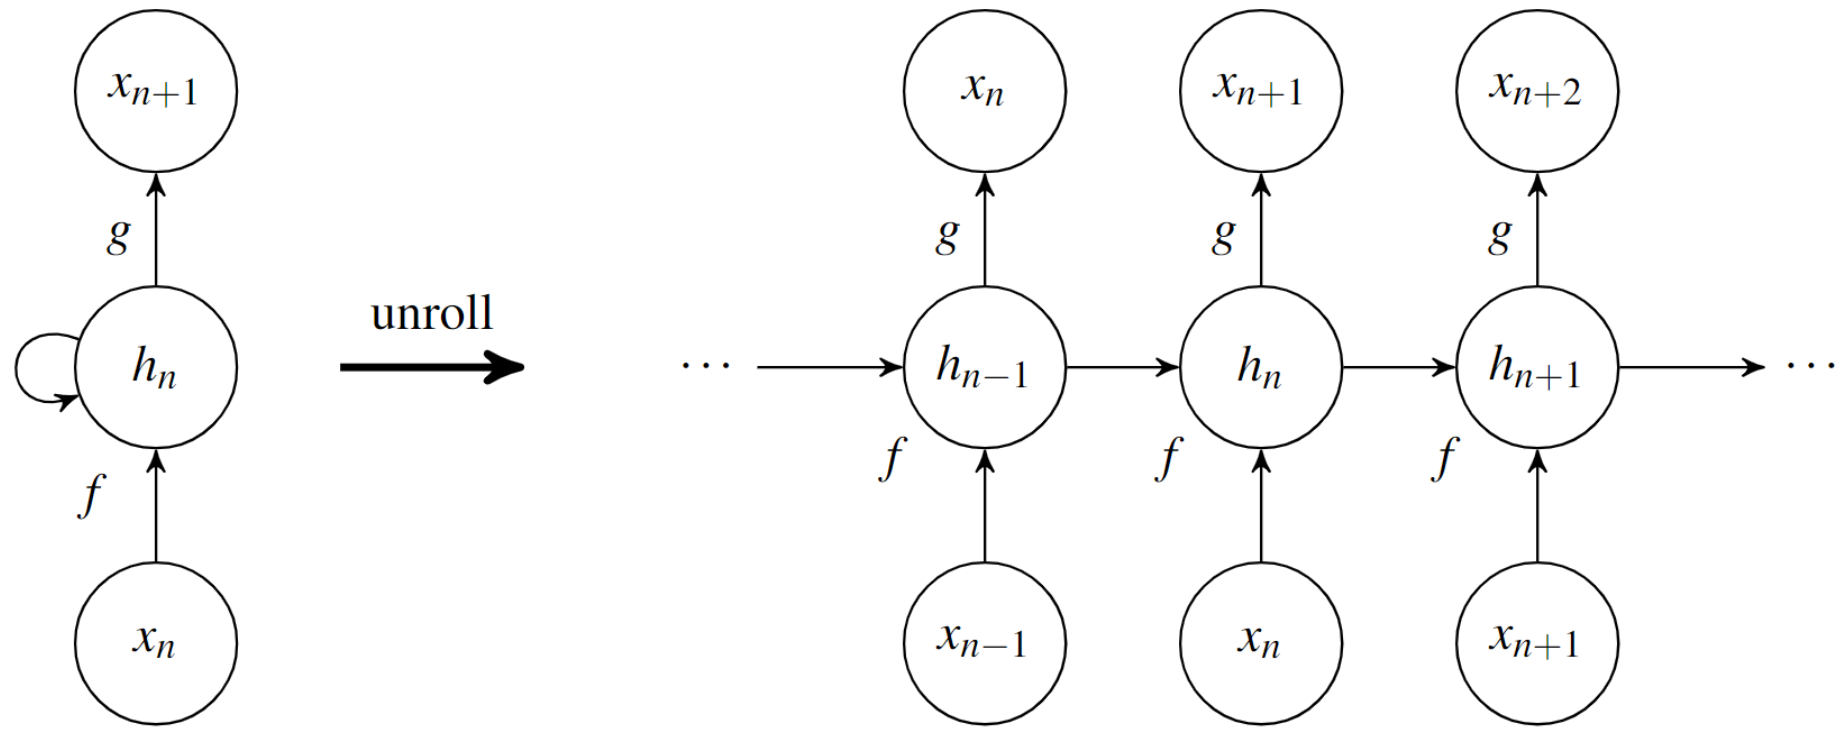
\includegraphics[width=12cm]{rnn.png}\\
  \caption{简单循环神经网络结构图}
  \label{fig:rnn}
\end{figure}

通过公式\ref{eq:rnn},\ref{eq:rnn1}可以明白,RNN的每一个时间步骤都会有一个新的输入,并且特定时间步骤的输出依赖于之前所有步骤的输入,这意味着时间步骤$N$时刻的损失函数的计算要回溯到时间步骤$1$,这一过程也称为\textit{基于时间的反向传播算法(backpropagation through time, BPTT)}\upcite{Sutskever:2013:TRN:2604780}。但是如果要处理的序列很长的话,经过多层的反向传播,BPTT会产生梯度消息或者梯度爆炸的问题,以至于无法从差的很远的时间步骤中感知上下文环境,使得RNN的训练变得非常麻烦,RNN这一明显的缺点也称为长期依赖问题。

\subsection{长短期记忆神经网络}

为了解决RNN的长期依赖问题,一些基于公式\ref{eq:rnn}的变形工作诞生,其中最广为人知的是长短期记忆网络(long short-term memory, LSTM)\upcite{LSTM1997}。LSTM通过精巧设计的记忆单元更换了RNN中的隐藏单元,其核心计算单元如图\ref{fig:lstm}所示。LSTM神经元内部通过精心设计的分别称为遗忘门、输⼊门、输出门的三个门结构来决定哪些信息更新到内部或者从内部去除。在遗忘门\eqref{forget_gate}当中,前一时间步的掩藏状态和当前时间步的输入经过Sigmoid函数非线性转换之后得到一个$[0,1]$之间的值,以表示需要遗忘信息的概率。在输入门\eqref{input_gate},\eqref{input_gate1}中,将当前时间步骤中的输入和前一时间步骤学习到的隐藏状态经过tanh激活函数的计算生成一些候选值,并通过Sigmoid函数的传递从候选值中选出一些进行更新。而输出门\eqref{output_gate}就决定了当前单元要输出哪些部分。LSTM通过如下的组合函数来更新隐藏单元的状态:
  \begin{align} 
  f_{t} &=\sigma(U_{f} x_{t}+W_{f}[h_{t-1}+ c_{t-1}] +b_{f}) \label{forget_gate}\\
  i_{t} &=\sigma(U_{i} x_{t}+W_{i}[h_{t-1}+ c_{t-1}]+b_{i}) \label{input_gate}\\  
  c_{t} &=f_{t} c_{t-1}+i_{t} \tanh (U_{c} x_{t}+W_{c} h_{t-1}+b_{c}) \label{input_gate1}\\ 
  o_{t} &=\sigma(U_{o} x_{t}+W_{o}[h_{t-1}+ c_{t}]+b_{o}) \label{output_gate}\\ 
  h_{t} &=o_{t} \tanh (c_{t}) 
  \end{align}
% \end{equation}

其中$\sigma(\cdot)$是Logistic Sigmoid激活函数;而$i$、$f$、$o$和$c$分别是输入门、遗忘门、输出门和隐藏层的激活向量;变量$b$表示偏置向量,例如$b_{f}$表示为遗忘门的偏置向量。$U$、$W$分别代表输入向量的权重和上一层输出的权重,例如在遗忘门中,$U_{f}$代表遗忘门输入向量$x_{t}$的权重,$W_{f}$代表上一个LSTM神经元输出$h_{t-1}$的权重。

\begin{figure}[htb]
  \centering
  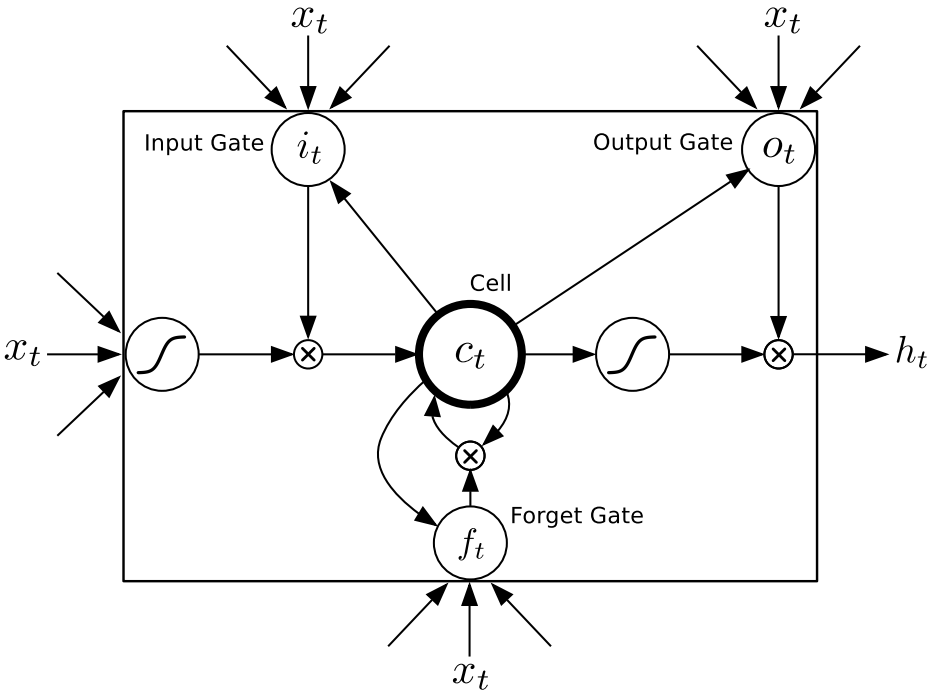
\includegraphics[width=12cm]{lstm.png}\\
  \caption{长短期记忆网络神经元结构图}
  \label{fig:lstm}
\end{figure}

\subsection{门控循环单元Gated Recurrent Unit}

由于LSTM在循环神经单元中增加了三个门结构,与RNN相比,在一个神经元当中要完成更多的复杂计算。当使用更大的网络的时候,训练时间相比RNN也将显著增加。为了减少训练的时间复杂度并同时保留LSTM对长期依赖关系的记忆能力,2014年Cho等人提出门控循环单元(Gated Recurrent Unit, GRU)\upcite{GRU2014}。与LSTM相似,GRU使用门结构建模单元内部信息的流动,不同的是,GRU将LSTM三个门减少为两个。GRU使用更新门来决定是否遗忘上时刻的信息或者记忆此时刻新的外部输入信息,其功能相当于组合了LSTM 中的输入门与遗忘门。使用重置门来决定如何将新的输入信息与内部已有放入记忆相结合。在$t$时刻GRU单元中更新门的状态表达式为:
$$
z_{t}^{j}=\sigma\left(U_{z} \mathbf{x}_{t}+W_{z} \mathbf{h}_{t-1}\right)^{j}
$$
其中,$\mathbf{x}_{t}$为第$t$个时间步骤的输入向量,$\mathbf{h}_{t-1}$中保存的是上一个时间步骤的信息。$U$,$W$是更新门当中输入向量与上一时间步信息的权重矩阵。$t$时刻GRU单元中重置门为:
$$
r_{t}^{j}=\sigma\left(U_{r} \mathbf{x}_{t}+W_{r} \mathbf{h}_{t-1}\right)^{j}
$$
结合更新门与重置门,整个GRU神经元在$t$时间步的内部状态更新为:
$$
z_{t}^{j}=\sigma\left(U_{z} \mathbf{x}_{t}+U_{z} \mathbf{h}_{t-1}\right)^{j}
$$
其中$\tilde{h}_{t}^{j}$为候选信息,表示当前记忆的内容,其计算表达式为:
$$
h_{t}^{j}=\left(1-z_{t}^{j}\right) h_{t-1}^{j}+z_{t}^{j} \tilde{h}_{t}^{j}
$$
单个GRU神经元的总体结构如图\ref{fig:gru}所示。

\begin{figure}[htb]
  \centering
  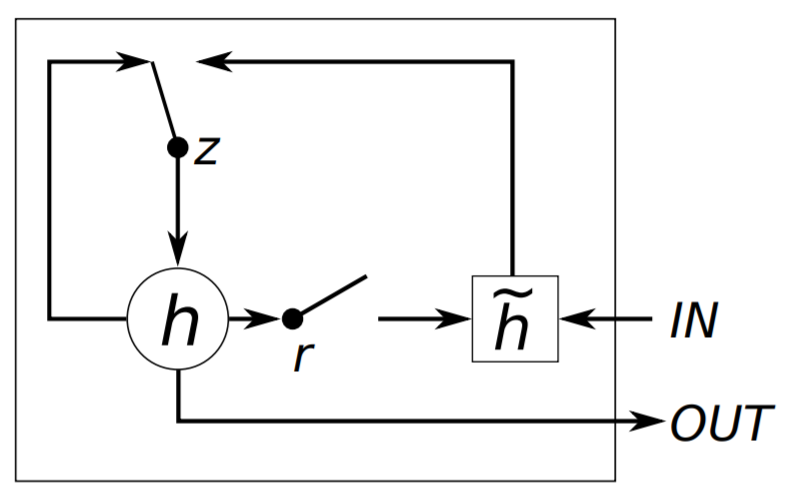
\includegraphics[width=12cm]{gru.png}\\
  \caption{门控循环单元神经元结构图}
  \label{fig:gru}
\end{figure}

\subsection{双向循环神经网络}

在自然语言处理的实体识别技术中,双向循环神经网络(Bidirectional recurrent neural networks, BRNN)\upcite{Schuster1997BidirectionalRN}弥补了单项循环神经网络对于上下文感知能力的不足,因为单向RNN预测下一个单词时使用的只是此单次出现之前的信息,而BRNN则从两个方向获取信息,上下文感知能力也就更强了。BRNN将隐藏层分为两个部分,前向状态层$\stackrel{\rightarrow}{h}$和反向状态层$\stackrel{\leftarrow}{h}$,其输出层的输入由$\stackrel{\rightarrow}{h}$和$\stackrel{\leftarrow}{h}$堆叠而成,其迭代公式如下:
\begin{align} 
  \vec{h}_{t} &= \sigma(U_{\vec{h}} x_{t}+W_{\vec{h} \vec{h}} \vec{h}_{t-1}+b_{\vec{h}}) \label{forword}\\
\stackrel{\leftarrow}{h}_{t} &= \sigma(U_{\stackrel{\leftarrow}{h}} x_{t}+W_{\stackrel{\leftarrow}{h} \stackrel{\leftarrow}{h}} \stackrel{\leftarrow}{h}_{t+1}+b_{\stackrel{\leftarrow}{h}}) \label{backword}\\
y_{t} &= W_{\vec{h} y} \vec{h}_{t}+W_{\stackrel{\leftarrow}{h}y} \stackrel{\leftarrow}{h}_{t}+b_{y} \label{stack}
\end{align}

BRNN的隐藏层结构如图\ref{fig:brnn}所示。
\begin{figure}[htb]
  \centering
  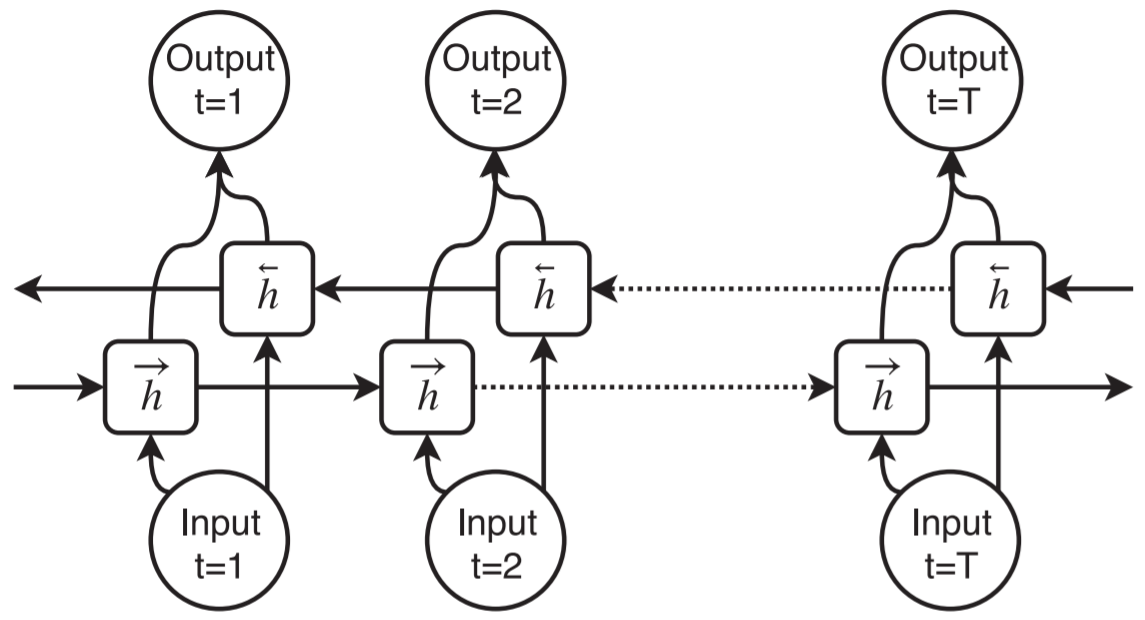
\includegraphics[width=12cm]{brnn.png}\\
  \caption{双向循环网络神经结构图}
  \label{fig:brnn}
\end{figure}

\subsection{时间卷积网络TCN}
卷积神经网络通常用于计算机视觉领域的图像特征提取,将其应用于序列建模需要对卷积神经网络的结构做出修改,目前将卷积神经网络运用于序列建模的最良好算法为2018年Shaojie Bai等人提出的时间卷及网络(Temporal Convolutional Network,TCN)\cite{TCN2018},本文在此把TCN作为CNN在序列建模领域的代表。

TCN由因果卷积(Causal Convolution)、扩张卷积(Dilated Convolution)和残差链接(Residual Connection)三部分构成。

\textbf{因果卷积}
在序列建模任务中,首先得保证输入序列与输出序列的长度一直,因此在TCN中使用的卷积结构是1维全卷机网络,其中每一个隐藏层的长度都与输入层长度相同,对于经过卷积过滤器计算的中间隐藏层,长度会减小,通过0填充的方式使其扩充到长度相等。如果直接对输入序列进行卷积操作的话,卷积操作将会是对序列的全局进行计算,这会导致信息泄露的问题,即在训练时让现在时刻知道了未来时刻的信息,而这种情况面对真实世界时是不可能发生的。为了防止训练时将未来时刻信息泄露到了现在时刻,因果卷积被引入。所谓因果卷积, 就是计算$t$时刻的输出时, 仅对前一层$t$时刻及之前的状态进行卷积。因果卷积等价于掩码卷积(masked convolution)\cite{DBLP:journals/corr/OordKK16},在输入序列上加上掩码把未来时刻的信息对现在时刻进行屏蔽。

\textbf{扩张卷积}
对于因果卷积,如果需要获得更大的感受野来捕获更长范围的序列的话需要很多层或者很大的过滤器,为了更加因果卷积的感受野,扩张卷积被引入与其结合。扩张卷积通过跳过部分输入来使过滤器能应用于比过滤器本身大小更大的范围,等同于通过0填充来扩大原先的过滤器。
Dilation convolution的运算如下:
$$
  F(s)=\left(\mathbf{x} *_{d} f\right)(s)=\sum_{i=0}^{k-1} f(i) \cdot \mathbf{x}_{s-d \cdot i}
$$
其中$\mathbf {x}$表示输入序列, $f$ 表示 过滤器filter, $d$ 是扩张因子,%
 $k$ 是过滤器大小,  $s-d\cdot i$意味着只对过去的状态作卷积。图\ref{fig:TCN}为结合了因果操作和扩张操作的卷积示意图。
\begin{figure}[htb]
  \centering
  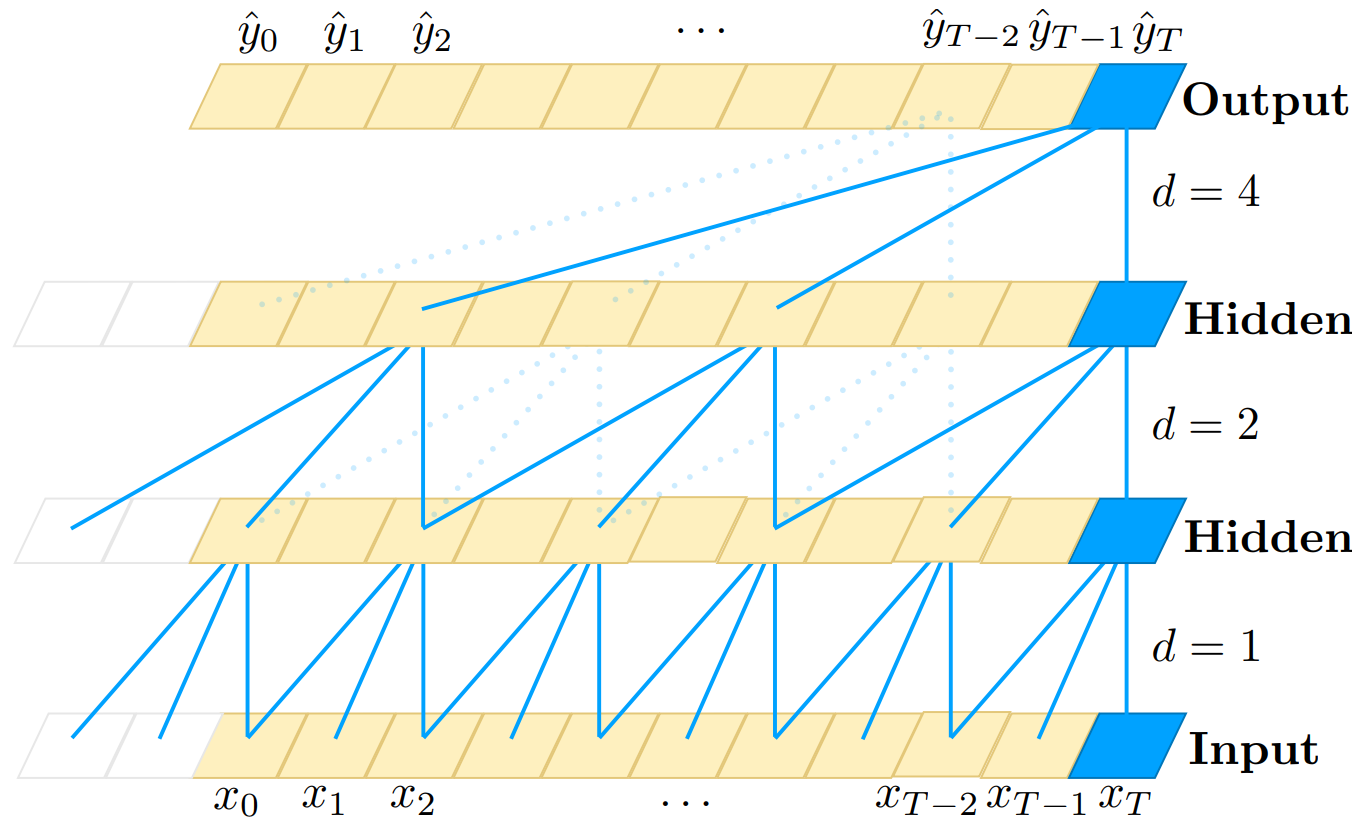
\includegraphics[width=\linewidth]{TCN.png}\\
  \caption{扩张因子分别为1,2,4和过滤器大小为3的扩张因果卷积网络结构图}
  \label{fig:TCN}
\end{figure}

\textbf{残差链接}
由于卷积神经网络对序列建模能记忆的时间步长度依赖于网络的深度,TCN为了获得更大的感受野,因此不得不增加网络的深度。为了使深层网络的训练不至于丢失浅层特征,残差连接是用来解决这个问题的常用办法,因此TCN结构中加入了残差连接以增加网络深度。
$$
  o=\operatorname{Activation}(\mathbf{x}+\mathcal{F}(\mathbf{x}))
$$
其中$\mathcal{F}(\cdot)$为残差结构略过的深层隐藏网络。残差网络通过建立输入与输出之间的捷径网络,使有效的浅层特征能够直接传递给输出层,避免了所有特征向量都必须经过深层隐藏网络的计算,保留了浅层有效特征,使得训练深层网络变得更加容易。


% \subsection{序列感知推荐算法评价指标}

\subsection{注意力机制}
在自言语言处理的机器翻译算法中,有一类端到端的模型有着出色的性能。
而为了说明深度学习中的注意力模型,就不得不先谈这一类端到端框架,因为目前大多数注意力模型都作为端到端框架下的一部分使用。
其中代表工作为2014年Ilya Sutskever等人提出的Seq2Seq\cite{DBLP:journals/corr/GehringAGYD17}模型,Seq2Seq有一个编码器(Encoder)和一个解码器(Decoder)构成
% \section{序列感知推荐}

Seq2Seq模型中把序列建模问题当做一个条件概率问题:
$$
  p\left(y_{i} | y_{1}, \ldots, y_{i-1}, \mathbf{x}\right)=g\left(y_{i-1}, s_{i}, c_{i}\right)
$$
其中$s_{i}$为Decoder中$i$时刻的状态,其计算公式为:$s_{i}=f\left(s_{i-1}, y_{i-1}, c_{i}\right)$,
$c_{i}$为该时刻状态的权重,其计算公式为$c_{i}=\sum_{j=1}^{T_{x}} \alpha_{ij} h_{j}$,其中$i$表示Encoder端的第$i$时刻输入。
$h_{j}$表示Encoder端的第$j$个输入的隐向量,$\alpha_{i j}$表示Encoder端的%
第$j$个输入与Decoder端的第$i$个输入之间的权值,表示源端第$j$个输入对目标端%
第$i$个输入的影响程度,$\alpha_{i j}$的计算公式如公式\ref{eq:attention}所示:
\begin{align}
  \alpha_{i j}=\frac{\exp \left(e_{i j}\right)}{\sum_{k=1}^{T_{x}} \exp \left(e_{i k}\right)} \label{attention}
\end{align} 
其中$e_{i j}=a\left(s_{i-1}, h_{j}\right)$

在公式6中,aij是一个softmax模型输出,概率值的和为1。eij表示一个对齐模型,用于衡量encoder端的位置j个词,对于decoder端的位置i个词的对齐程度(影响程度),换句话说:decoder端生成位置i的词时,有多少程度受encoder端的位置j的词影响。对齐模型eij的计算方式有很多种,不同的计算方式,代表不同的Attention模型,最简单且最常用的的对齐模型是dot product乘积矩阵,即把target端的输出隐状态ht与source端的输出隐状态进行矩阵乘。常见的对齐计算方式如下:


\section{本章小结}


%!TEX root = ../document.tex
\chapter{基于双向长短期记忆网络的序列感知推荐算法}

推荐系统面临的问题主要有两大类:评分预测和项目推荐。所以在推荐领域根据用户的历史活动记录预测%
用户下一次行为可能会选择什么项目也是一个重要的问题。在许多在线网站和应用程序当中,如在线电子%
商务、新闻或视频推荐网站、音乐或广播电台,它们都需要为用户提供一个杰出服务来推荐用户在未来可能%
会喜欢的东西。现有的推荐系统主要关注于找出用户或项目的近邻集,或者利用隐式或显式信息(如标签、%
评论、物品内容、用户属性)来提升近邻感知能力。然而,却少有工作利用数据当中的时序属性来直接构建推荐系统。%
在本篇论文中,我们发现数据的序列中其实包含着许多有价值的且激动人心的信息,以视频网站为例,一个用户看%
了纪录片《河西走廊》第一集《使者》之后,接下来看的另一个节目很有可能会是《河西走廊》第二集《通道》。甚至早在%
2011年举办的Recsys推荐系统大会上,来自音乐应用Pandora\footnote{\url{www.pandora.com}}的研究%
人员给出的演讲上都提到了许多用户听音乐具有时序特点。%

在某些特别的应用场景下,常规的推荐系统甚至无法起作用。现有的推荐系统都需要分析用户的数据,因此每个%
网站和应用的使用到需要让用户完成注册以及登录,然而用户每次使用网站或者应用的服务时都不一定会愿意%
登录,这种场景下对匿名用户的推荐显然挑战更大,常规的推荐策略显然无法起作用,基于匿名用户本地浏览器%
和缓存的会话所蕴含的序列进行推荐则显现出很重要的实践意义与价值。

\section{算法框架描述}

为了挖掘许多现有算法忽视掉的用户行为序列特征,本文提出了使用神经网络来对用户的序列进行建模的思路。%
我们的模型(\textit{BiLSTM4Rec})主要由五个部分组成,分别以此是嵌入层、循环结构、全连接层、池化层和输出预测层。其整体框架%
结构如图\ref{fig:structer}所示。

\begin{figure}[htb]
  \centering
  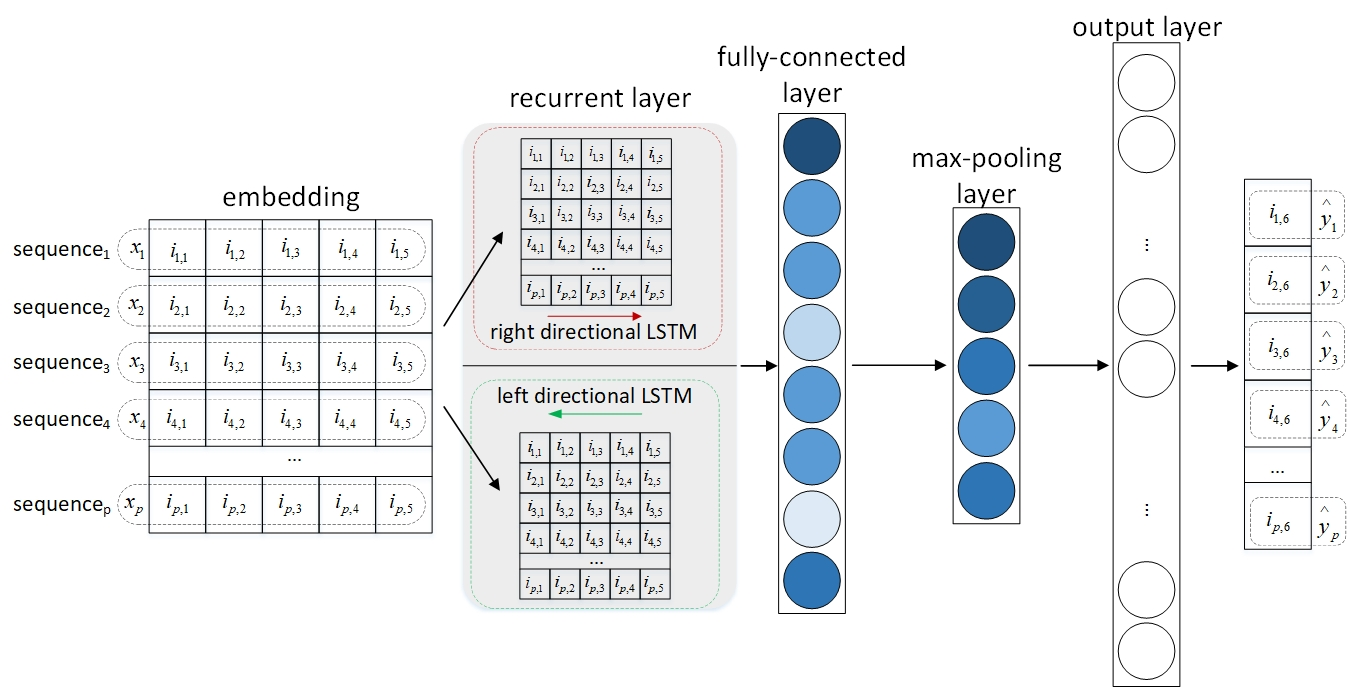
\includegraphics[width=\linewidth]{structer.jpg}\\
  \caption{基于双向循环神经网络的序列推荐算法BiLSTM4Rec框架图}
  \label{fig:structer}
\end{figure}

% \section{基于双向长短期记忆网络的序列感知推荐模型}
\subsection{目标问题定义}

序列感知推荐与传统的单类协同过滤推荐是有很大不同的,序列感知推荐的主要目标是预测用户下一步将会%
点击什么,而且利用数据仅仅包含用户当前历史行为的序列集合,而不接触为用户设置的长期偏好属性。%
接下来我们将定义序列感知这一问题的形式。%

在序列感知推荐当中,我们定义$\mathbb{U}= \left \{ u_{1},u_{2},...,u_{N} \right \}\label{eq}$%
代表不同的用户集合,定义$\mathbb{I}= \left \{ i_{1},i_{2},...,i_{M} \right \}$代表在所有序列%
中出现过的不同物品集合,$s_{u}^{t}\in \mathbb{I}$表示用户$u$在时间刻$t$点击某一个物品的记录,%
该记录对应的物品包含在物品集合$\mathbb{I}$当中。对于每一个用户$u$,%
都记录一个按照数据诞生时间戳顺序排列的用户点击记录%
序列$\mathbb{S}_{u}=\left \{ s_{u}^{1},s_{u}^{2},...,s_{u}^{t-1},s_{u}^{t} \right \}$%
序列感知推荐的目标是预测下一次点击行为,也就是做出$t+1$时刻的推荐$s_{u}^{t+1}$。在序列感知推荐%
模型当中,对于序列$s$,模型的输出是所有候选物品对象可能被点击的概率$\hat{y}$,而概率最大的$K$个%
输出所对应的候选物品将作为推荐项目给到用户。%
%
%
%
%

\subsection{嵌入层}

我们使用用户消费历史的最近几个序列当做特征,用户消费的最后一个物品当做标签,来构建一个超多分类%
的有监督学习模型。因此,在特征工程阶段,我们需要将原始序列特征数据转换为计算机容易处理的向量形式%
并且与标签映射。One\_hot编码是用来表达离散特征的最常用的向量表达形式,然而One\_hot编码的向量会遇%
到高维和稀疏的问题。如果我们使用One\_hot编码来处理具有1000个类别的特征,那么每个特征会被一个拥%
有1000个数字的向量来表示,但其中999个数字会是0。在一个大规模数据集中,就计算效率而言这种方式是%
不可取的。

例如对序列$s_{1},s_{2},s_{3},s_{4},s_{1}$进行One\_hot编码的话,将会得到如图%
\ref{fig:one_hot}的形式
\begin{figure}[htb]
  \centering
  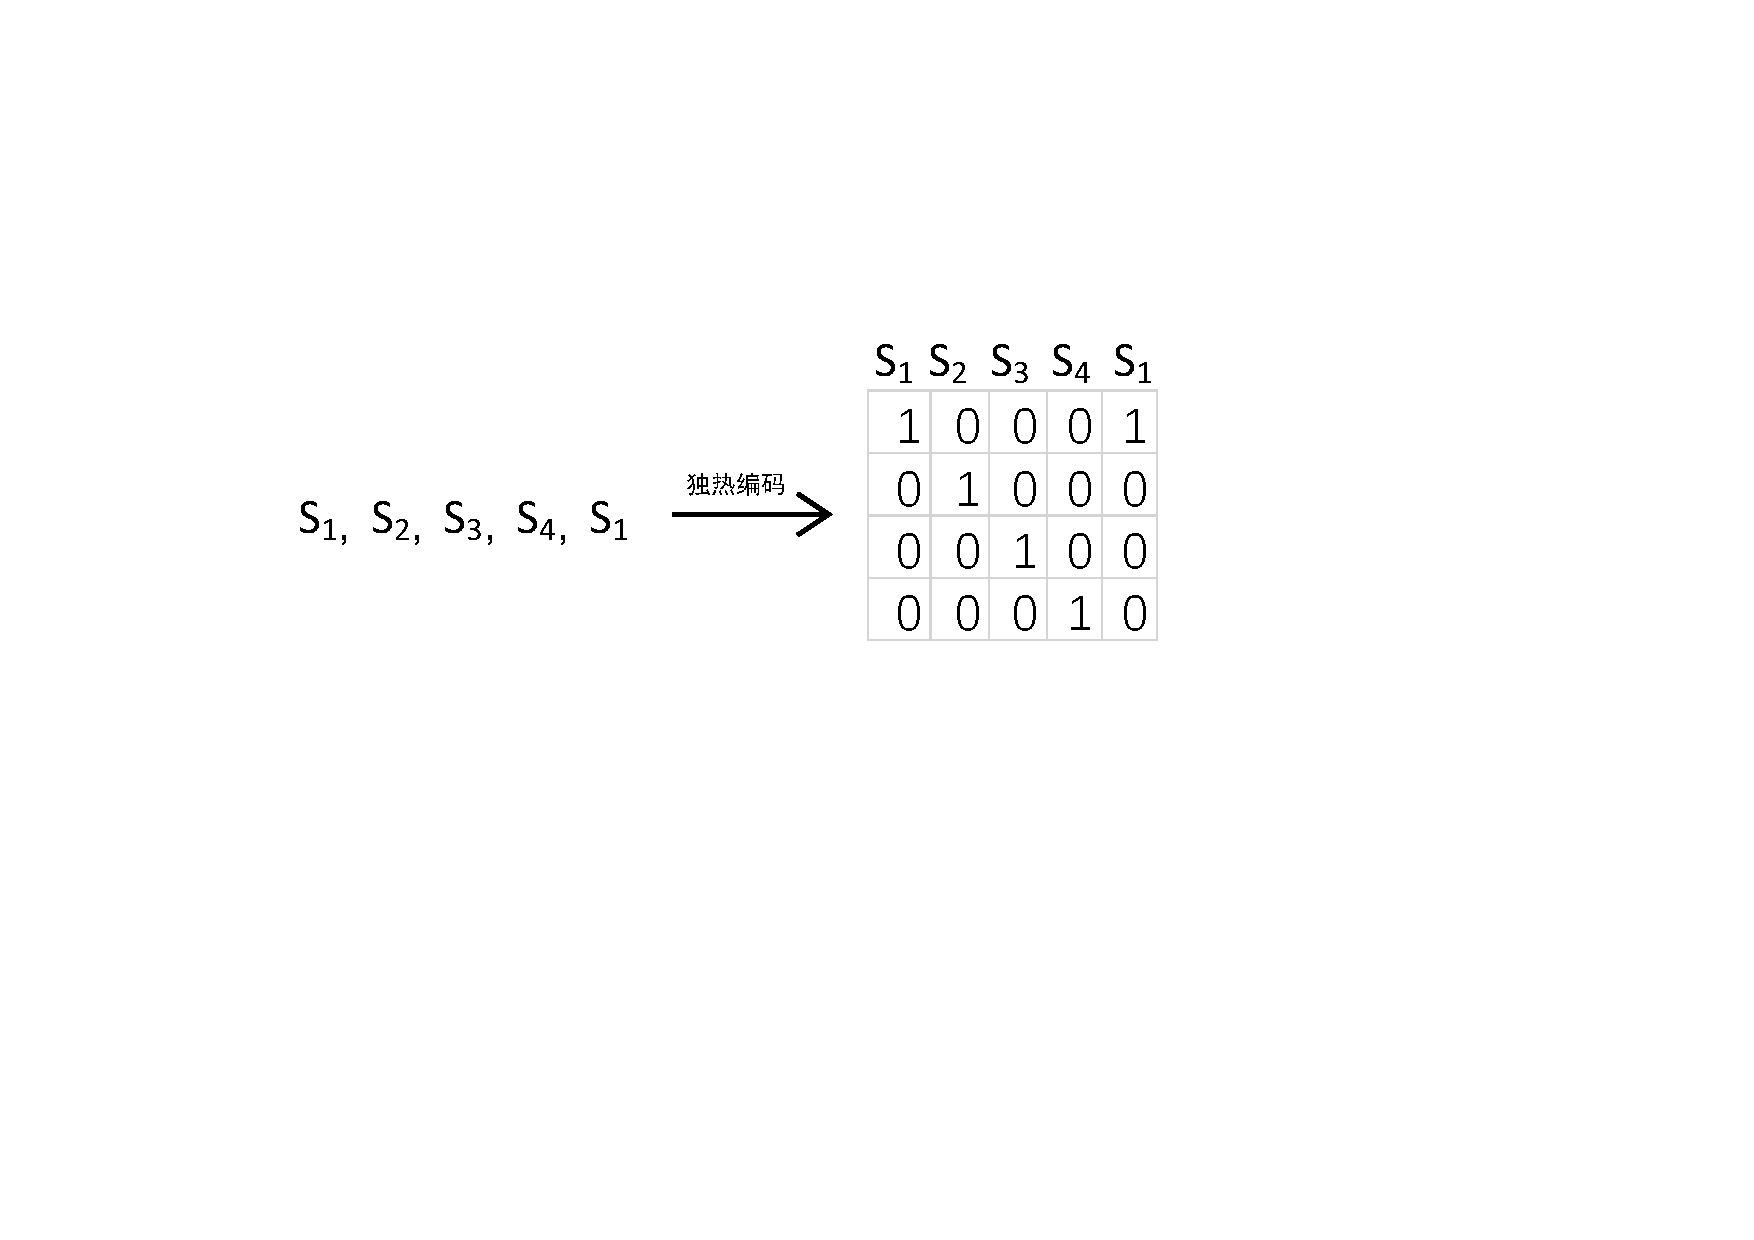
\includegraphics[width=0.6\linewidth]{one_hot.pdf}\\
  \caption{序列独热编码示意图}
  \label{fig:one_hot}
\end{figure}

而词嵌入技术在自然语言处理领域大放异彩,我们可以借用词嵌入技术\upcite{Mikolov:2013:DRW:2999792.2999959},也构造一个嵌入矩阵来%
得到比One\_hot形式小得多的向量结构:
\begin{align}
e(I_i) = EI_i
\end{align}
其中$E\in \mathbb{R}^{|e|\times |M|}$, $|e|$是嵌入层的大小,$|M|$是训练集中不同项目的数量。%
所以$e(I_i)$是$I_i$的嵌入表达,其是一个具有$e$个实数的稠密矩阵。与一个 $|M|\times |M|$大小的%
One\_hot编码形式相比,我们的序列嵌入矩阵的大小为$|e|\times |M|$,当处理大数据集时,这显著减小%
了内存消耗。
\begin{figure}[htb]
  \centering
  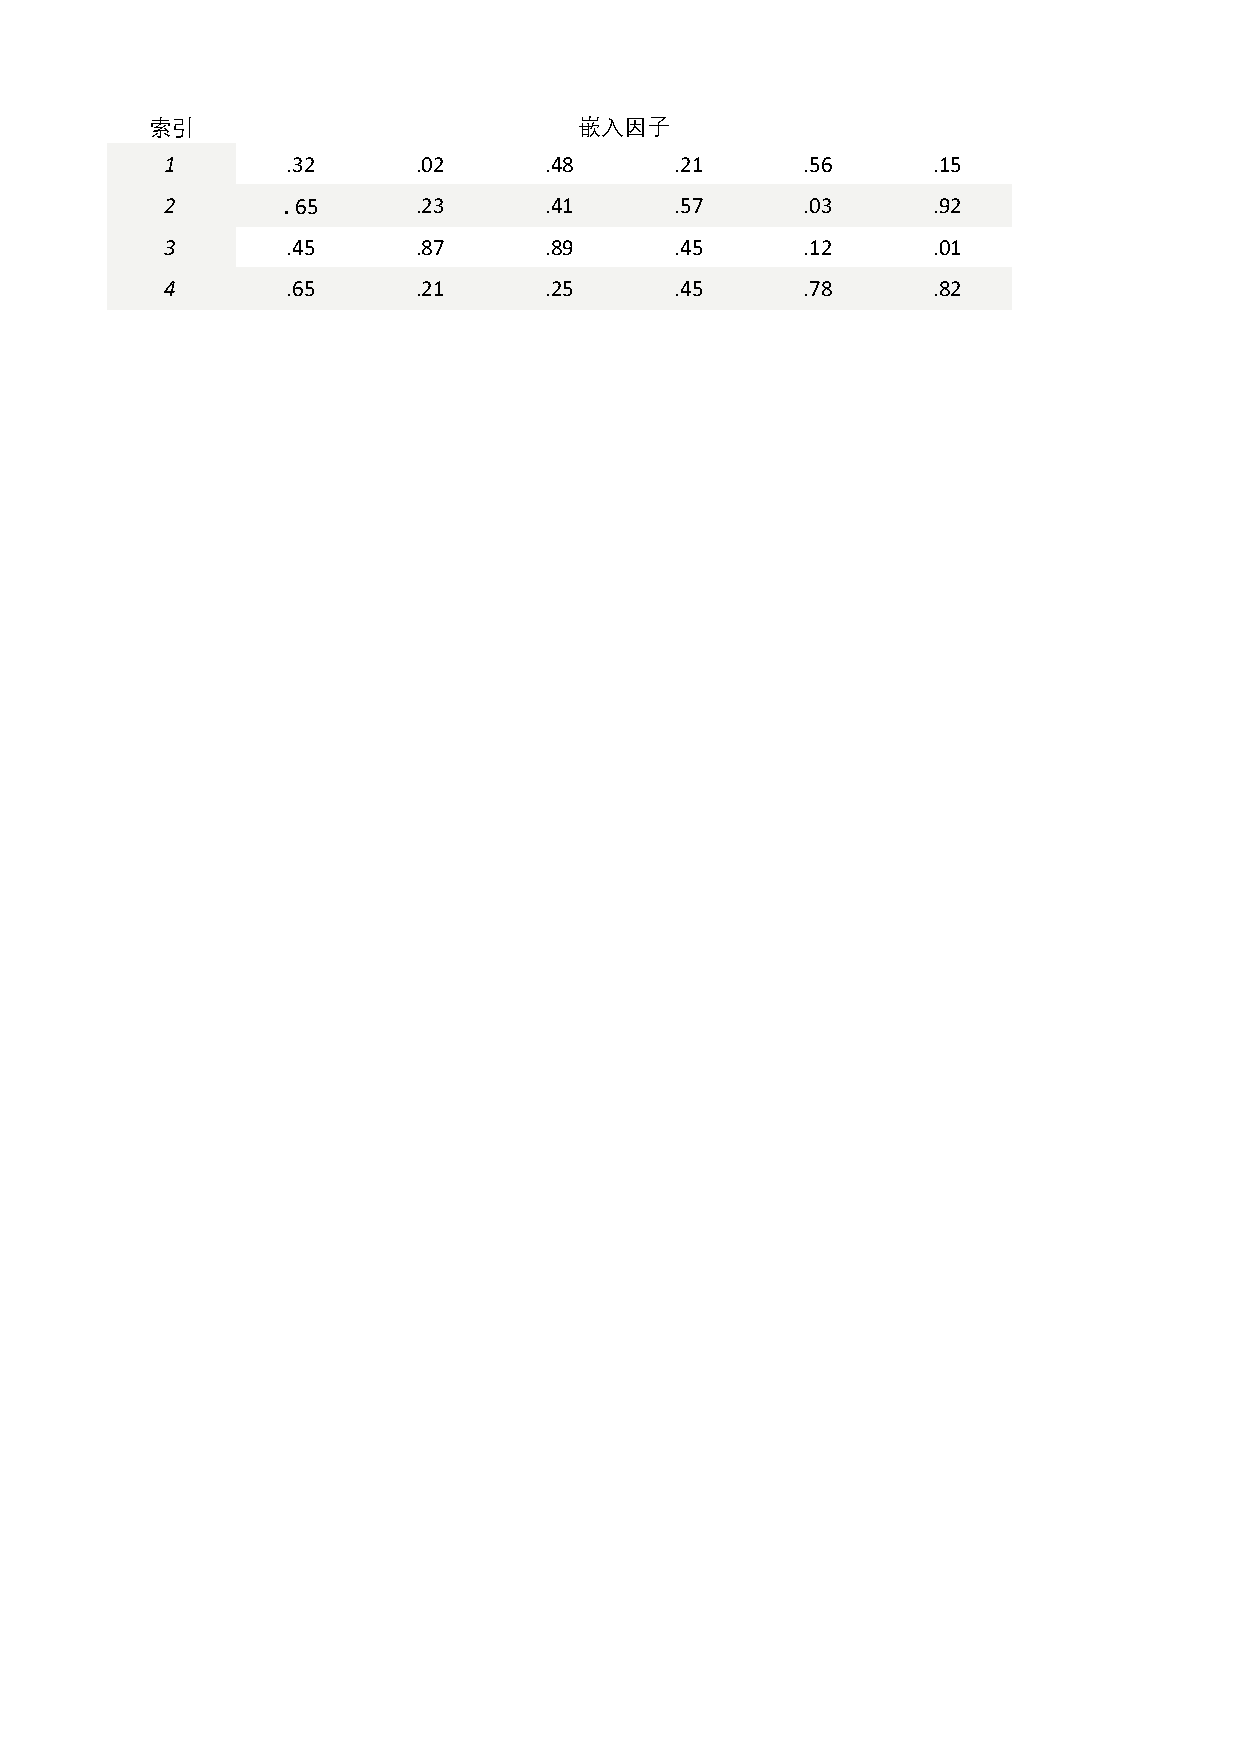
\includegraphics[width=\linewidth]{embedding.pdf}\\
  \caption{序列嵌入编码示意图}
  \label{fig:embedding}
\end{figure}
Embedding嵌入编码中并不是每一个物品ID都会被一个向量来代替,而是被替换为用于查找嵌入矩阵中向量的%
索引。其次这种方法面对大数据时也可有效计算。由于在深度神经网络的训练过程中嵌入向量也会被更新,还%
可以探索在高维空间中哪些物品之间具有彼此相似性。

\subsection{用户短期兴趣学习}

我们通过结合用户$u$在$t$时刻消费的项目$I_{u}^{t}$和其先后的项目来表达用户在此时刻的兴趣。行为序列帮助我们更精确地揭示了用户的短期兴趣。在这个推荐系统中,我们使用了一个双向的长短期记忆神经网络构建的循环结构来捕捉用户短期的兴趣变化。

我们定义$h_{b}(I_{i})$ 为用户他在消费物品$I_i$之前的兴趣,$h_{a}(I_{i})$为用户消费物品$I_i$之后的兴趣。$h_{b}(I_{i})$和$h_{a}(I_{i})$都是具有$|h|$个实数的稠密向量。$W^{(b)}$是隐藏层的权重矩阵,用来继承用户之前的兴趣状态,矩阵$W^{(cb)}$用来结合前一个物品的嵌入表达,$\sigma$是一个非线性激活函数,因此通过学习表达式$h_{b}(I_{i})$来学习用户消费物品$I_i$之前的兴趣。同理,用户消费物品$I_i$之后的兴趣通过学习表达式$h_{a}(I_{i})$来学习
。所有用户的初始兴趣使用同样的参数$h_{b}(I_{1})$,用户消费历史中的最后的兴趣则共享参数$h_{a}(I_{n})$。
\begin{align}
h_{b}(I_{i})=\sigma (W^{(b)}h_{b}(I_{i-1})+W^{(cb)}e(I_{i-1})) \\
h_{a}(I_{i})=\sigma (W^{(a)}h_{a}(I_{i+1})+W^{(ca)}e(I_{i+1}))
\end{align}
通过以上公式,学习用户某个时刻之前和之后的兴趣,将它们和用户当前消费物品的嵌入矩阵集合来表达此时刻用户的临时兴趣状态,其结合形式如下:
\begin{align}
x_{i}=[h_{b}(I_{i});e(I_{i});h_{a}(I_{i})]
\end{align}
所以通过使用大量用户的历史行为序列$\left \{ i_{1},i_{2},...,i_{n-1},i_{n} \right \}$,如果我们的模型学习到了某个用户消费物品$i_{n-1}$时的临时兴趣$x_{n-1}$,他将更有可能得到一个物品推荐$i_{n}$.双向循环结构能够对序列的前向扫描中捕获所有的$h_b$,反向扫描则捕获了所有的$h_a$。当训练集中所有的临时兴趣状态$x_i$都被捕获之后,运用一个线性转换与tanh激活函数将结果送到下一层。
\begin{align}
y_{i}^{(2)}=tanh(W^{(2)}x_{i}+b^{(2)})
\end{align}
$y_{i}^{(2)}$是潜在的兴趣向量,其中的每一个兴趣向量将通过上面权重和参数的更新来决定影响用户消费序列中最重要的因素。

\subsection{流行趋势学习}
当用户消费项目的所有序列被计算完之后,接下来应用一个最大池化层:
\begin{align}
y^{(3)}=\max_{i=1}^{n}y_{i}^{(2)}
\end{align}
最大池化通过应用一个最大过滤器到上层代表的非重叠子区域,有了池化层,模型的参数或权重迅速减小了,这样也能减小上层输入的空间维度,减小计算消耗。通过对全局序列属性的捕获最大输出层能在用户的这个历史记录里找到那些最流行的序列组合。模型的最后一层就是常规的输出层了:
\begin{align}
y^{(4)}=W^{(4)}y^{(3)}+b^{(4)}
\end{align}
输出层通过应用一个softmax激活函数到$y^{(4)}$来转换成下一个类别的输出概率:
\begin{align}
p_{i}= \frac{e^{y_{i}^{(4)}}}{\sum_{k=1}^{n}e^{y_{k}^{(4)}}}
\end{align}

\subsection{模型的训练}

将模型训练过程中所有需要更新的参数定义为$\theta $。
\begin{equation}
\theta=  \left \{ E,b^{(2)},b^{(4)},h_{b}(B_{1}),h_{a}(B_{n}),W^{(2)}, W^{(4)},\right.\\
\left.W^{(b)},W^{(a)},W^{(b)},W^{(cb)},W^{(ca)} \right \} \\
\end{equation}

模型训练的优化目标是最小化交叉熵损失函数:
\begin{equation}
\mathcal{L}(y,S,\theta )=-\sum_{u\in \mathbb{U}}[y_{u}\log p(y_{u}|S_{u},\theta)+(1-y_{u})\log (1-p(y_{u}|S_{u},\theta ))]
\end{equation}

\section{复杂度分析}

在嵌入层当中,主要包含一个矩阵的向量想乘操作,这一部分的时间复杂度是$O(n)$。在双向长短期记忆网络中,网络的主体是LSTM,其时间复杂度为$O(n\cdot d^{2})$,$n$表示序列的长度,$d$表示嵌入层因子的维度。而双向LSTM的时间复杂度我们可以知道为$2\cdot O(n\cdot d^{2})$,最大池化层的时间复杂度为$O(n)$,全连接层的时间复杂度为$O(n)$,整个模型是上述这些结构的串联,所以整个基于双向循环神经网络的序列推荐算法的时间复杂度为$O(n\cdot d^{2})$。相比于基于用户的协同过滤算法(UBCF)\upcite{Resnick:1994:GOA:192844.192905}的时间复杂度$O(n_{u}^{2})$和基于物品的协同过滤(IBCF)\upcite{Sarwar:2001:ICF:371920.372071}时间复杂度$O(n_{i}^{2})$,其中$n_{u}$表示用户数量,$n_{i}$表示物品数量。与其相比,序列长度$n$和嵌入维度$d$存在这样的关系:$n_{u}> n_{i}\gg d> n$,所以基于双向循环神经网络的序列推荐算法在选择合适的序列长度和嵌入维度大小时面对大数据处理的压力时还是可以接受的。

\section{算法实现}
\begin{algorithm}[H]%[htbp]
	\caption{基于双向长短期记忆网络的序列感知推荐算法}
	\label{alg:bi-lstm}
		\begin{algorithmic}[1]
			\REQUIRE 用户序列数据:$S$;序列长度:$maxLen$; 最大物品数:$maxNum$
			\ENSURE 推荐结果:$Items$
			\STATE $sequence \leftarrow S$, 其中$sequence=\{seq_{1}, seq_{2}...seq_{n}\}$
			\IF {$len(sequence) >= maxLen$}
				\STATE 选取序列最后的N物品:$sentences_{lastn} \subseteqq sequence$
			  	\STATE $items \leftarrow sequence_{topn}$,其中 $items=\{word_{1}, word_{2}...word_{m}\}$
			  \FOR{each $i \in [1,maxLen]$}
			    \STATE 将每个序列的物品ID编码到嵌入矩阵:$E = Embedding_{seq_{i}}$
			  \ENDFOR
			  
			\ELSE
				\STATE continue
			\ENDIF
			\FOR{each $i \in [1, maxLen]$}
				\STATE $output_{right}$ = LSTM(E)
				\ENDFOR
			\FOR{each $i \in [maxLen, 1]$}
				\STATE $output_{left}$ = LSTM(E)
				\ENDFOR
			\STATE $output$ = $[output_{right}; output_{left}]$
			\STATE $output$ = $maxpolling(output)$
			\STATE $NextItem = SoftMax(output) $
			\RETURN $NextItem$
		\end{algorithmic}
\end{algorithm}

\section{本章小结}

本章节主要介绍本文提出的一个针对用户下一个点击推荐的新颖神经网络推荐模型BiLSTM4Rec,其利用双向长短期记忆网络来对用户按照时间先后点击物品的历史记录进行序列建模,挖掘隐藏在序列当中的用户短期兴趣变化,来精确地对用户下一个可能感兴趣的物品做出推荐。通过对大规模物品ID进行矩阵嵌入压缩处理,借助该时序推荐算法,能够取得比传统协同过滤更高效更精确地短期推荐策略。


%!TEX root = ../document.tex
\chapter{基于自注意力机制的序列感知推荐}

\section{问题的提出}
在多个不同的机器学习领域,例如图像描述、机器翻译、阅读理解、摘要生成还有一些其他的应用上,已经证明注意力机制是有明显效果的%
这一机制背后的重要思想是影响序列输出的因素只与序列中某些重要信息相关,而无需过多关注其他无用的信息。这一机制的命名受到人类视觉系统中视觉焦点的启示,所以称为注意力机制。

2017年NIPS大会上谷歌发表了一个完全用注意力机制构建的机器翻译框架\textit{Transfomer}\upcite{NIPS2017_7181},到达了当时最好的效果。
\section{算法框架描述}

在基于循环神经网络的序列感知推荐系统方面,由于循环神经网络本身的特性也带来了性能上面的一些缺陷。由于循环神经网络的结构,当前神经元的输入有上一个神经元的输出,反向传播梯度更新时,下一个神经元的梯度更新也需要上一个神经元计算完再开始,这一串行的性质限制了循环神经网络的训练速度,特别是当需要使用更深的循环神经网络的时候。而由于自注意力机制完全抛弃了循环神经网络的串行结构而依然能捕获数据的序列关系,近来已成为序列建模领域的研究热点。
使用注意力机制的另一好处是基于注意力的方法在推荐可解释性方面也更好说明。%
因此在这一部分,我们为了进一步的提升基于双向循环神经网络的序列感知推荐算法,本章基于编码器解码器框架,选用自注意力机制作为编码器和解码器的特征提取器,来建模用户短期行为模式的依赖因素,本文中将此模型称为\textit{Transformer4Rec},其整体框架结构如图\ref{fig:transformer}所示。

\begin{figure}[htb]
  \centering
  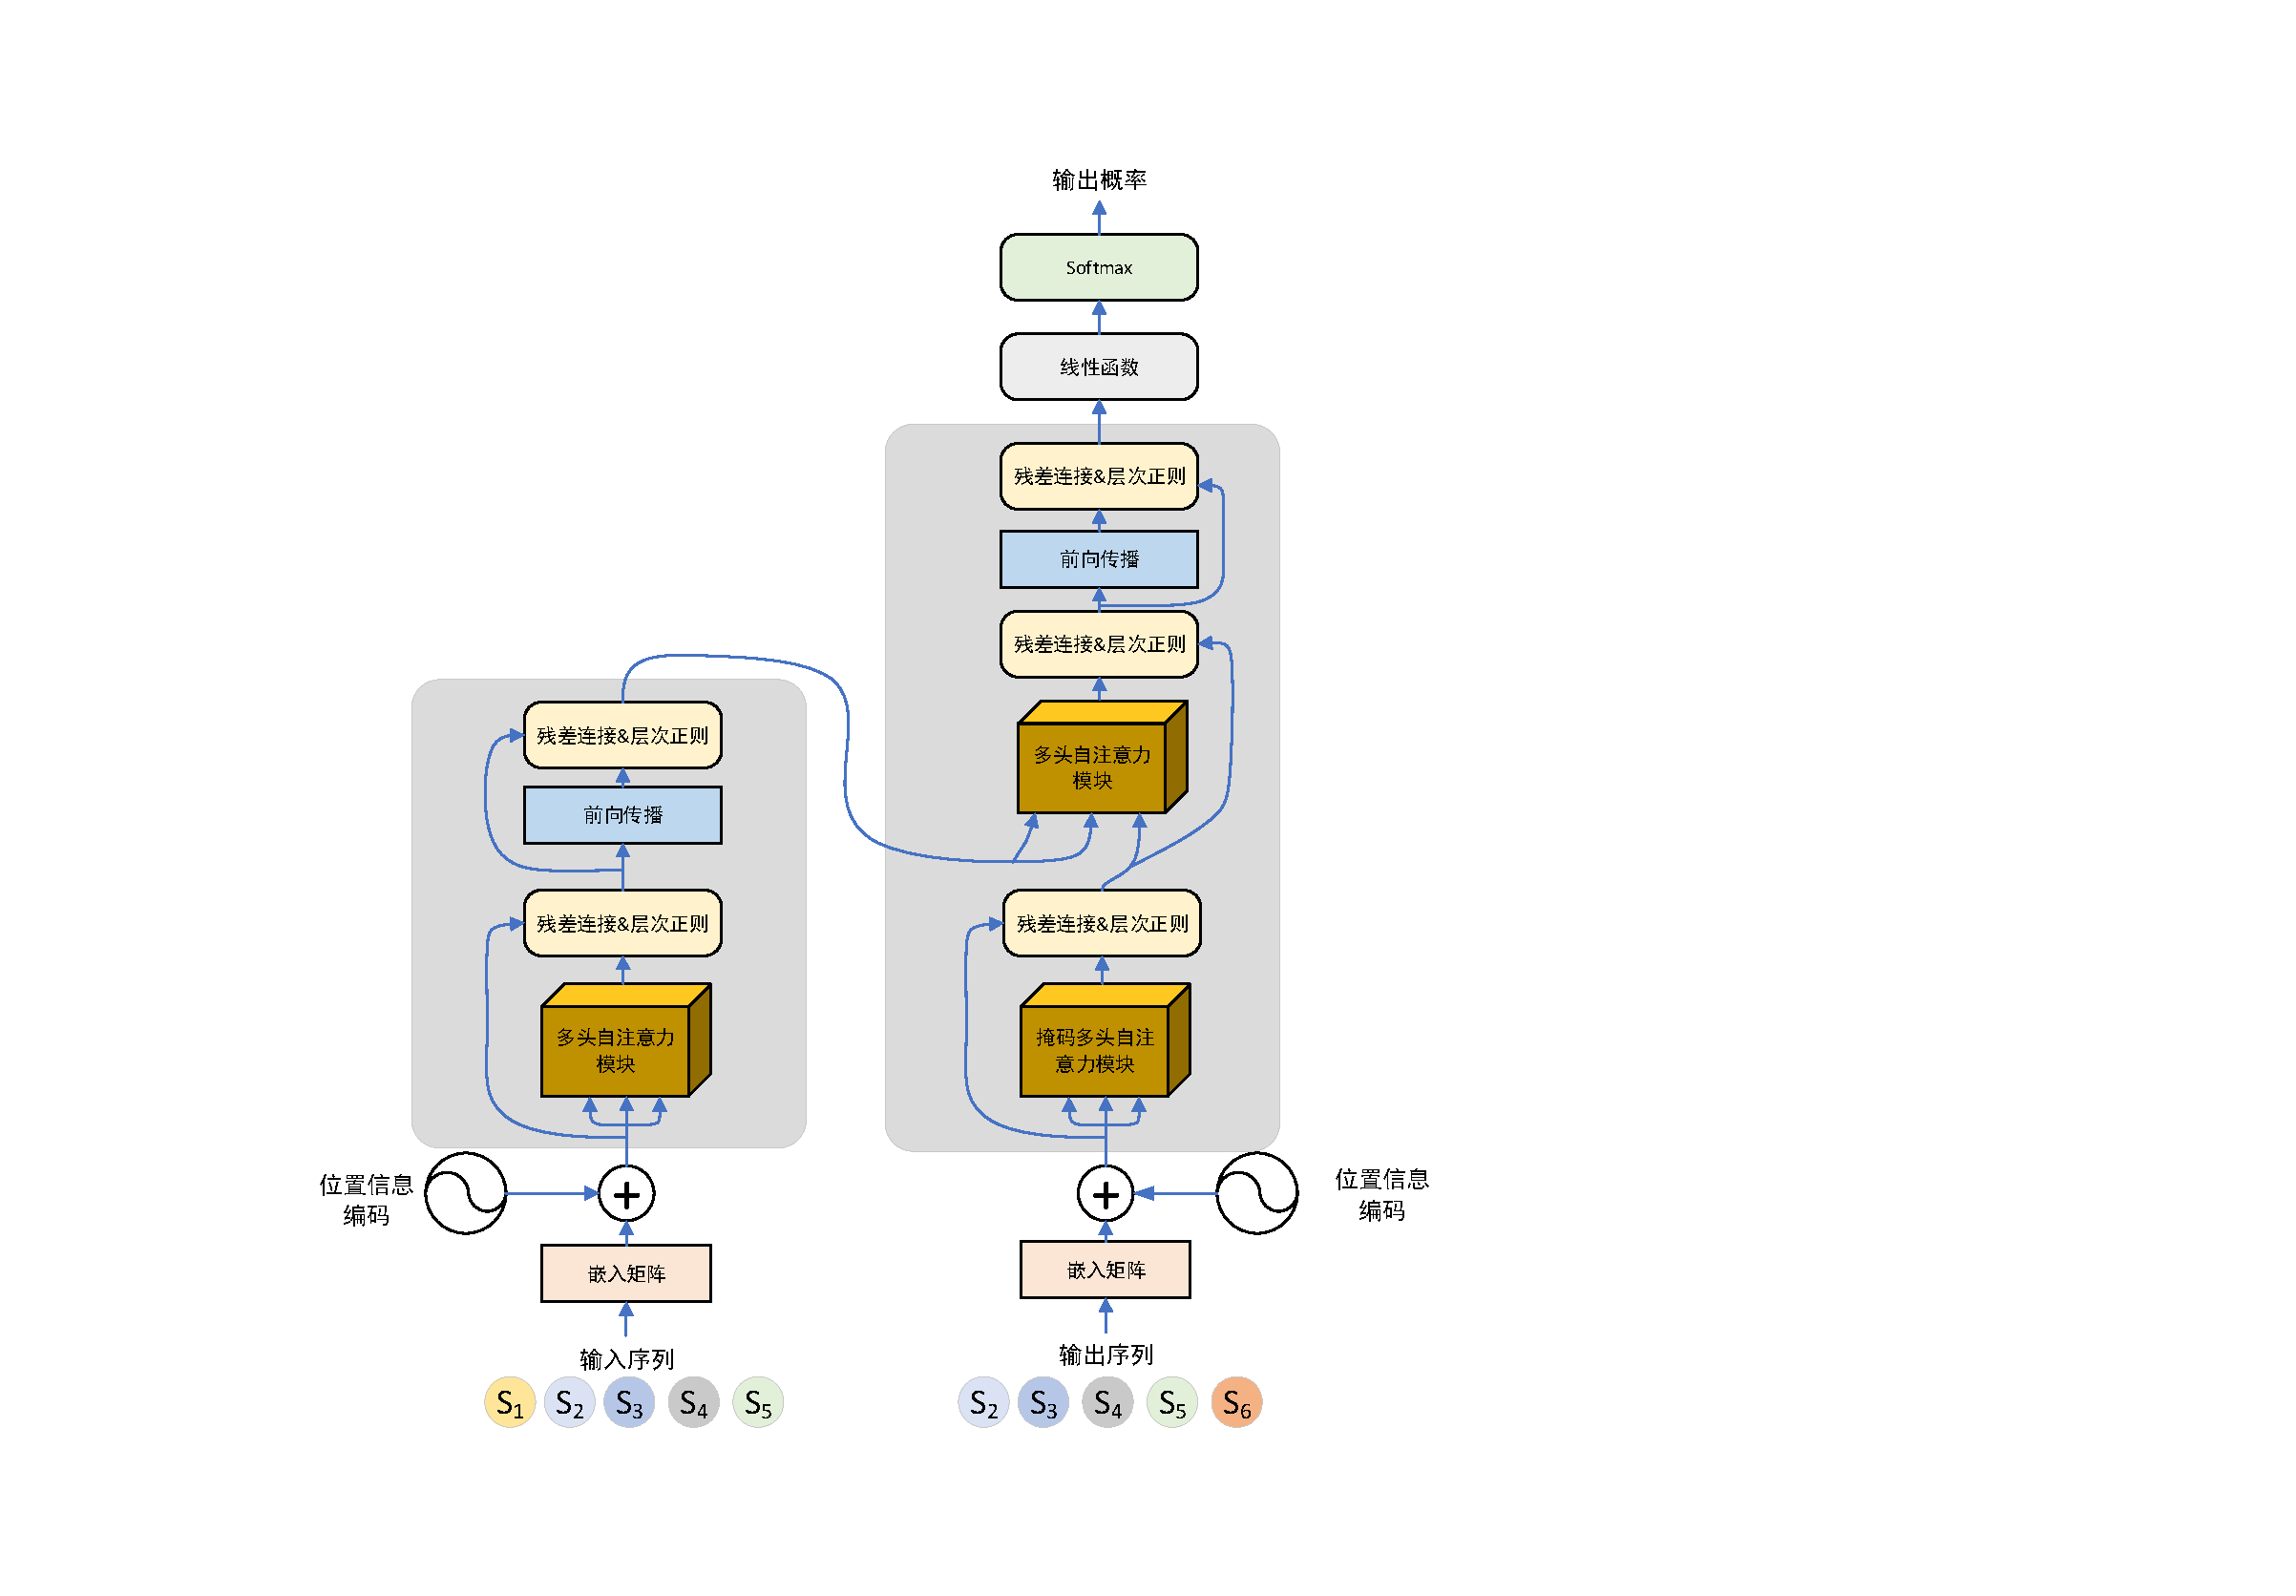
\includegraphics[width=\linewidth]{transformer.pdf}\\
  \caption{基于自注意力机制的序列推荐算法Transformer4Rec框架图}
  \label{fig:transformer}
\end{figure}

% \section{基于自注意力机制的序列感知推荐模型}
\subsection{目标问题定义}

与第三章中基于双向长短期记忆网络的序列感知推荐模型问题一样,我们定义$\mathbb{U}= \left \{ u_{1},u_{2},...,u_{N} \right \}\label{eq}$%
代表不同的用户集合,定义$\mathbb{I}= \left \{ i_{1},i_{2},...,i_{M} \right \}$代表在所有序列%
中出现过的不同物品集合,$s_{u}^{t}\in \mathbb{I}$表示用户$u$在时间刻$t$点击某一个物品的记录,%
该记录对应的物品包含在物品集合$\mathbb{I}$当中。对于每一个用户$u$,%
都记录一个按照数据诞生时间戳顺序排列的用户点击记录%
序列$\mathbb{S}_{u}=\left \{ s_{u}^{1},s_{u}^{2},...,s_{u}^{t-1},s_{u}^{t} \right \}$%
序列感知推荐的目标是预测下一次点击行为,也就是做出$t+1$时刻的推荐$s_{u}^{t+1}$。在序列感知推荐%
模型当中,对于序列$s$,模型的输出是所有候选物品对象可能被点击的概率$\hat{y}$,而概率最大的$K$个%
输出所对应的候选物品将作为推荐项目给到用户。%

\subsection{嵌入层}

序列中的物品ID不具有实际数学意义,因此不能把ID编码直接%
传输给计算机进行计算,但为了使计算机能够以较少的资源消耗而感知不同的物品身份,这里同样不使用One\_hot编码%
而使用与基于双向长短期记忆网络的序列感知算法一样的嵌入矩阵\upcite{Mikolov:2013:DRW:2999792.2999959}来对物品ID进行处理:
$$
e(I_i) = EI_i
$$
其中$E\in \mathbb{R}^{|e|\times |M|}$, $|e|$是嵌入层的大小,$|M|$是训练集中不同项目的数量。%
所以$e(I_i)$是$I_i$的嵌入表达,其是一个具有$e$个实数的稠密矩阵。

\textbf{位置信息嵌入层}

由于在利用自注意力方法构建的模型当中,没有了循环和卷积结构,因此抛弃了项目之间的序列信息,但%
用户的短期兴趣关注点隐藏在序列之中,为了使我们的模型能够捕捉到序列变化信息,必须将序列中物品%
的相对或者绝对位置信息加入到模型当中去。位置编码有可学习形式(learned)和固定参数形式%
(fixed)\upcite{DBLP:journals/corr/GehringAGYD17}。这里我们使用了与%
\textit{Transfomer}\upcite{NIPS2017_7181}一样的方式,在模型输入的嵌入层中加入物品序列的固定参数形式“位置编码”,%
即位置信息嵌入层。我们使用正弦和余弦函数并结合不同频率将物品的固定位置编码传递给模型,位置编码%
的一个维度对应于正弦曲线上的一个值,从而形成从$2\pi $到$10000 \cdot  2\pi$的几何级数波长,%
这些信号作为额外的信息加入到输入(或输出)中以表达时间的流逝,使模型能够%
感知到当前正在处理的是输入(或输出)序列的哪个部分。:
\begin{align}
  PE(t,2e) &= \sin (t/10000^{2e/d_{model}}) \label{eq:sin}\\
  PE(t,2e+1) &= \cos (t/10000^{2e/d_{model}}) \label{con}
\end{align}
\begin{figure}
\centering
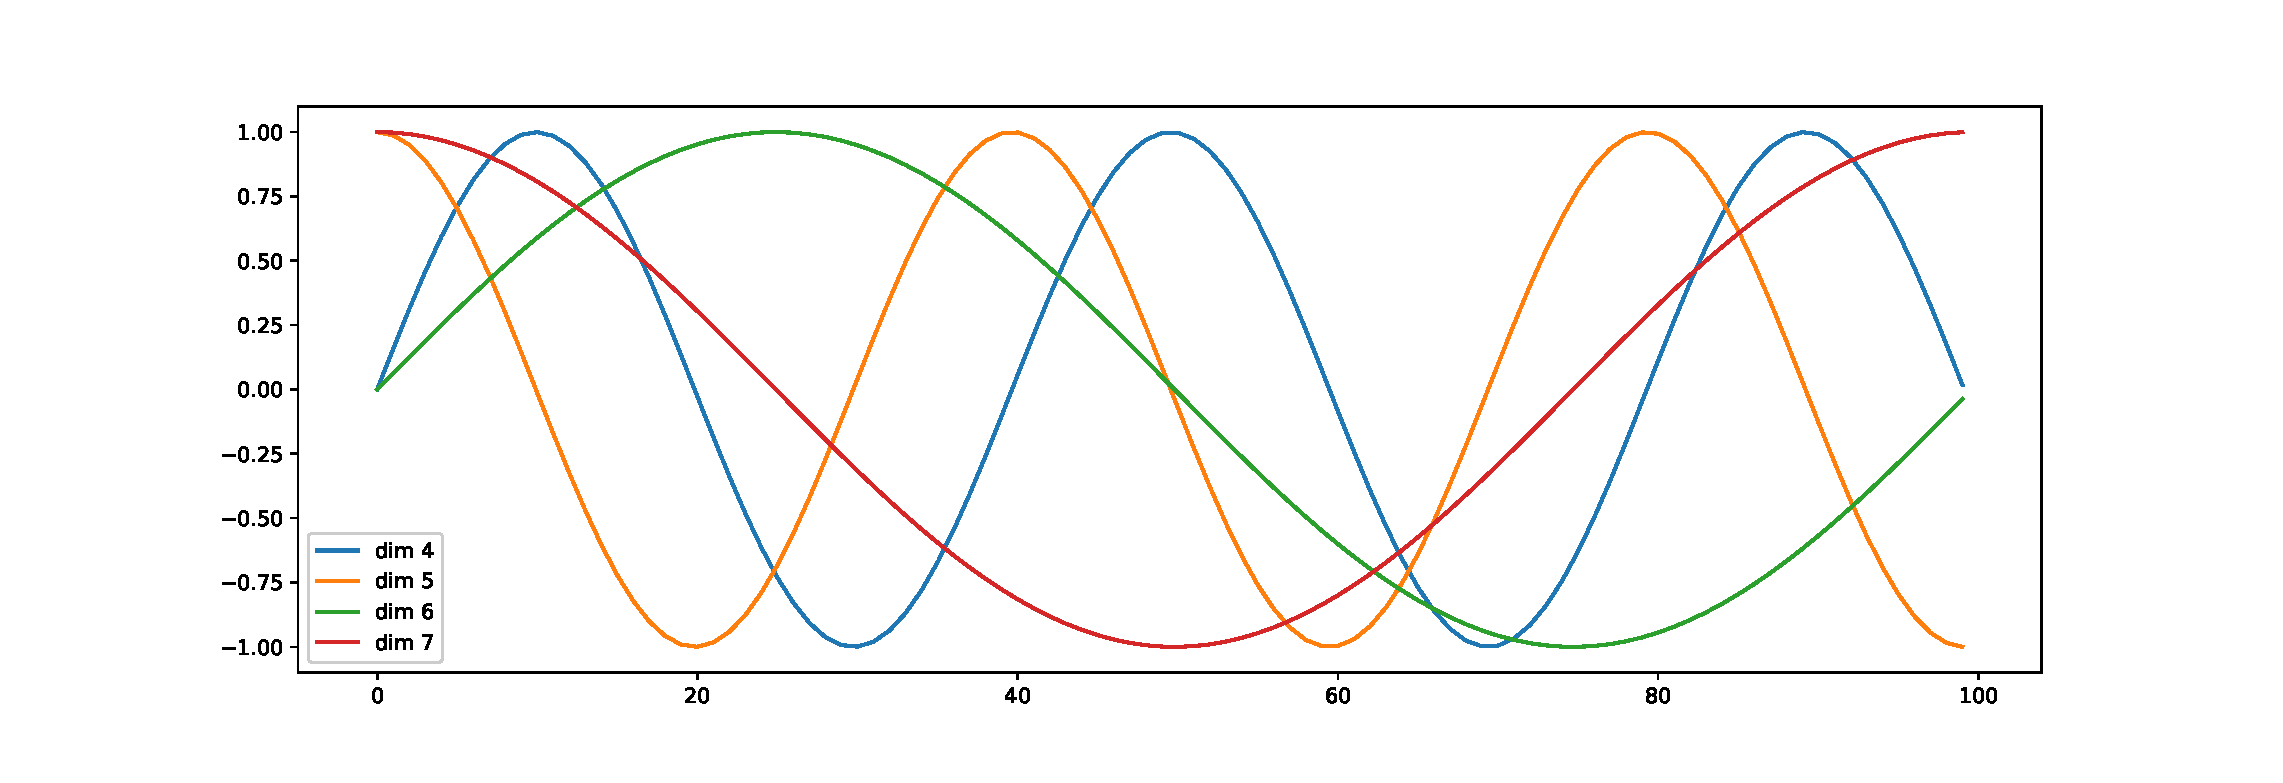
\includegraphics[height=4cm,width=14cm]{pe.eps}
\caption{使用不同维度大小的位置编码波形图}
\label{pe}
\end{figure}

其中$t$就是位置信息,表示该物品出现在序列中的第$t$个时间步骤,$e$是位置嵌入层的维度。图\ref{fig:pe}显示,不同的位置嵌入层维度大小,位置编码波形图具有不同的波长。由于位置信息嵌入层与嵌入层有相同的维度$|e|$,因此可以把两者相加起来构成我们最终的输入嵌入层$\widehat{\mathbf{E}}$:
\begin{equation}
	% \label{equ:chap04:embedding}
	\label{fig:pe}
	\widehat{\mathbf{E}}=\left[ \begin{array}{c}{\mathbf{E}_{s_{1}}+\mathbf{PE}_{1}} \\ 
	{\mathbf{E}_{s_{2}}+\mathbf{PE}_{2}} \\ 
	\cdots \\
	{\mathbf{E}_{s_{n}}+\mathbf{PE}_{n}}\end{array}\right]
\end{equation}

\subsection{编码器解码器框架}
编码器解码器(Encoder-Decoder)框架\upcite{D14-1179,DBLP:journals/corr/GehringAGYD17}是自然语言处理中常用的一种序列生成框架,其常用来构建机器翻译模型。Encoder-Decoder框架由一个解码器(Encoder)和一个编码器(Decoder)构成,
Encoder用来处理输入序列$x_{1},x_{2},x_{3},\cdots ,x_{t-1},x_{t}$,将输入序列处理成语义向量,Decoder用来生成输出序列$y_{1},y_{2},y_{3},\cdots ,y_{t-1},y_{t}$,将处理过的语义向量转换成输出序列。Encoder与Decoder的构建可以根据任务的不同选取具有不同特性的CNN/RNN/BRNN/GRU/LSTM算法。


但在我们的序列推荐框架中,考虑序列中的每一个输入节点,其期望的输出应为其序列中直接后继节点,因此我们可以根据这一性质构建一个Encoder-Decoder框架,如图所示:

\begin{figure}
\centering
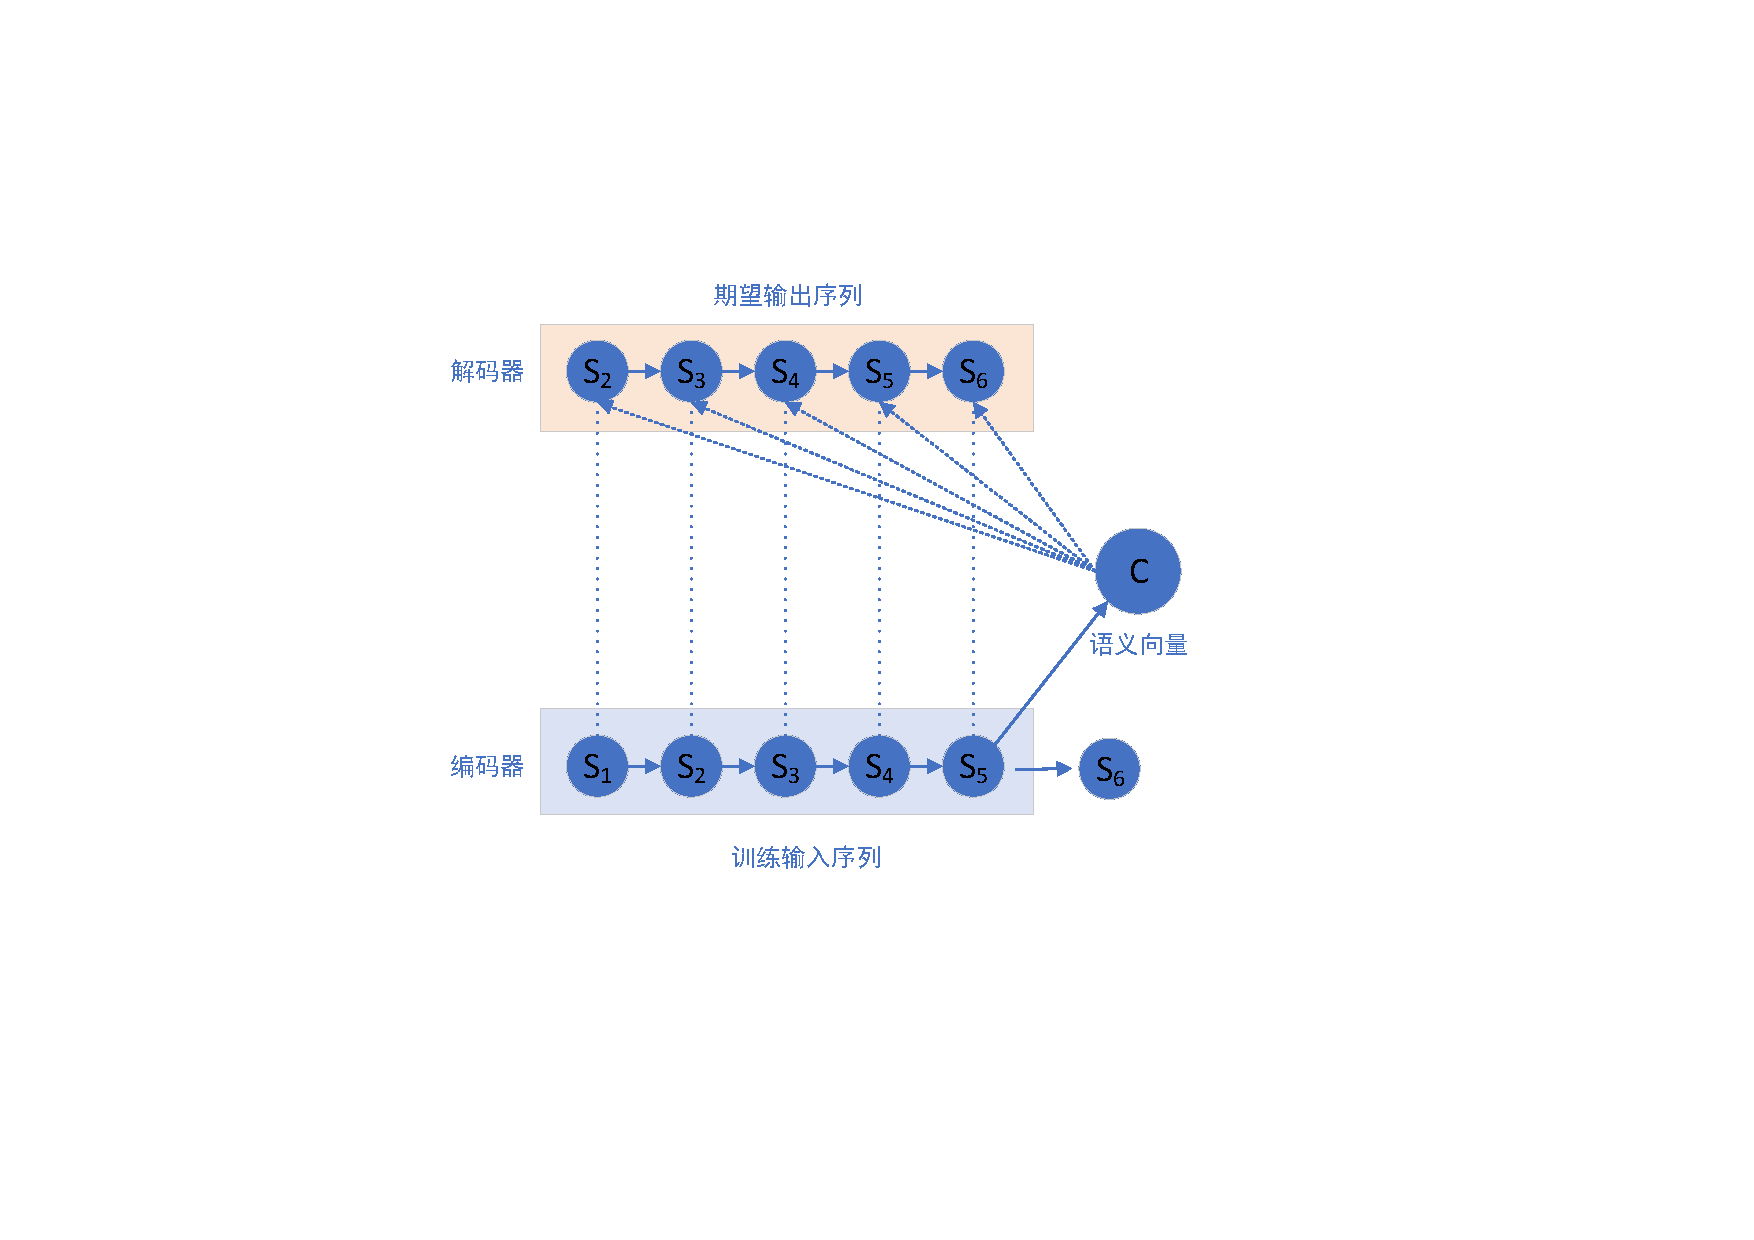
\includegraphics[height=6cm]{encoder-decoder.pdf} %,width=8cm
\caption{Encoder-Decoder框架结构示意图}
\label{encoder}
\end{figure}


输入节点$s_{1}$,其对应的期望后继节点应为$s_{2}$,输入节点$s_{5}$,其期望的后继节点应为$s_{6}$。由于循环神经网络自身结构导致的难以并行训练问题,Encoder和Decoder的特征提取下我们准备选用自注意模型,下面对自注意模型的构建方式进行了介绍。

\subsection{自注意力模块}

自注意力方法是一种特殊的注意力机制,已有在各种任务上的成功应用。与最简单的注意力方法通过对%
整个语境学习得到有限的知识表示不同,自注意力方法即使面对相隔距离较远的两个元素,其依然能%
保存上下文中的序列信息并且捕获这两个元素在序列上的关系。因此我们这里使用自注意力方法来捕获%
用户历史行为中的序列特征。

构建自注意力模块的基本单元由\textit{缩放点乘注意力Scaled Dot-product Attention}构成,%
一个自注意力模块的输入由\textit{查询(query)},\textit{键(key)}和\textit{值(value)}%
三部分组成。自注意力模块的输出是模块中\textit{值(value)}的加权和得来,而这里的权重矩阵则有%
\textit{查询(query)}和其对应的\textit{键(key)}决定。

我们用$Q$表示\textit{查询(query)}向量,用$K$表示\textit{键(key)}向量,用$V$表示%
\textit{值(value)}向量,向量中的每一行代表一个物品。首先,我们通过使用共享参数的非线性%
变换将\textit{查询}和\textit{键}投影到同一空间:
\begin{align} 
	Q^{\prime} &=\operatorname{ReLU}(W_{Q}\widehat{\mathbf{E}}) \\ 
	K^{\prime} &=\operatorname{ReLU}(W_{K}\widehat{\mathbf{E}})
\end{align}

其中$W_{Q}$,$W_{K}$分别是\textit{查询}和\textit{键}向量的权重矩阵,%
得到$Q^{\prime}$和$K^{\prime}$之后我们就可以通过如下形式得到\textit{值(value)}%
的权重矩阵:
\begin{align} 
	V^{\prime}=\operatorname{softmax}(\frac{Q^{\prime} {K^{\prime}}^{T}}{\sqrt{d}})
\end{align}
其中$\sqrt{d}$为缩放因子,为了避免点乘之后出现过大的值导致softmax的输出被推到梯度消失的%
位置,因此加上缩放因子来优化矩阵点乘。于是Self-Attention模块的输出就可以计算出来了:
\begin{align} 
	\mathbf{S}=\mathrm{SA}(\widehat{\mathbf{E}})=\text { Attention }(W_{Q}\widehat{\mathbf{E}}, W_{K}\widehat{\mathbf{E}}, W_{V}\widehat{\mathbf{E}}) = V^{\prime}\widehat{\mathbf{E}}
\end{align}

\textbf{多头注意力机制Multi-Head Attention}
{}
与其只让单个Self-Attention模块来学习$d$维的\textit{查询(query)},\textit{键(key)}和\textit{值(value)},可以通过集成学习的方法,让多个Self-Attention模块分别学习不同位置子空间的表达,由于随机初始化的不同,每个Self-Attention模块的关注点将会有所差异,所以每个Self-Attention模块可以分别学习到三个不同的$d_{k}$维的\textit{查询(query)}、$d_{k}$维的\textit{键(key)}和$d_{v}$维的\textit{值(value)}向量。每个Self-Attention模块有了\textit{查询(query)}、\textit{键(key)}和\textit{值(value)}之后,就能得到$d_{v}$维的输出。而Multi-Head Attention是多个Scaled Dot-product Attention的并行叠加,因此Multi-Head Attention的计算复杂度与Scaled Dot-product Attention相当,但是却获得了更好的泛化性能。因此这部分Multi-Head Attention的计算方式如下:
\begin{align} 
	\text { MultiHead }(\widehat{\mathbf{E}}) =\text { Concat }[\mathrm{SA}_{1}(\widehat{\mathbf{E}}), \ldots, \mathrm{SA}_{h}(\widehat{\mathbf{E}})] W^{O}
\end{align}
其中$h$表示我们将$h$个Self-Attention模块并联堆叠在一起得到Multi-Head Attention模块。

\begin{figure}[!htb]
   \begin{minipage}{0.48\textwidth}
     \centering
     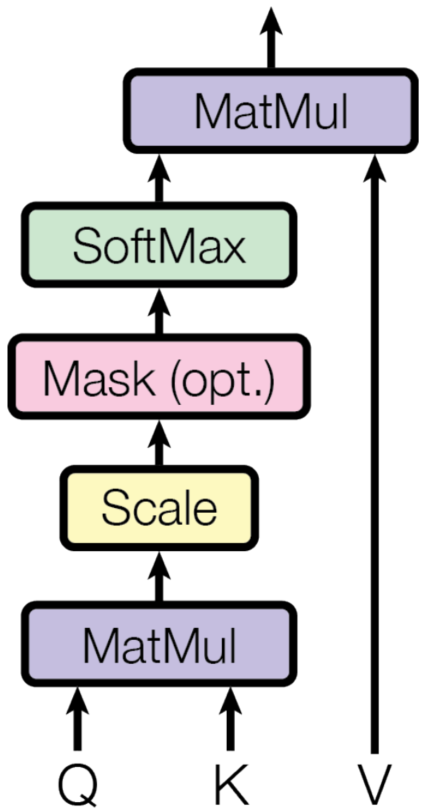
\includegraphics[height=6cm]{Scaled_Dot-Product_Attention.png} % ,width=\linewidth
     \caption{Scaled Dot-Product Attention缩放点乘注意力结构图}
     \label{Fig:Scaled_Dot-Product_Attention}
   \end{minipage}\hfill
   \begin {minipage}{0.48\textwidth}
     \centering
     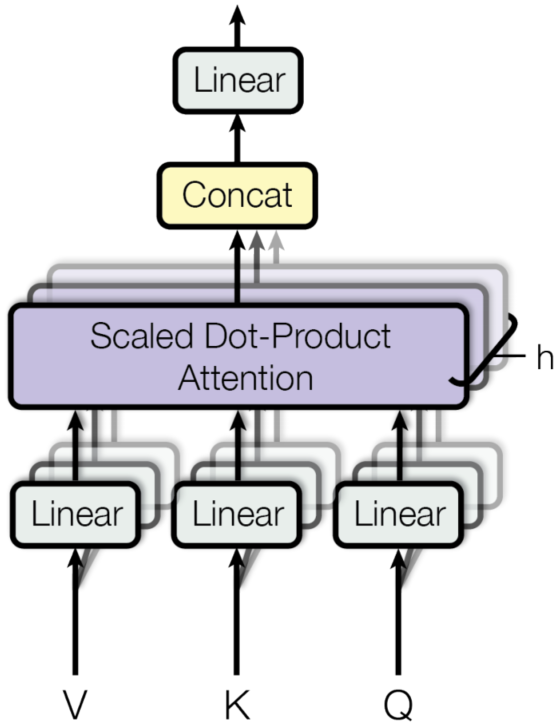
\includegraphics[height=6cm]{Multi-Head_Attention.png} % ,width=\linewidth
     \caption{Multi-Head Attention多头注意力模块结构图}
     \label{Fig:Multi-Head_Attention}
   \end{minipage}
   % \caption{BiLSTM4Rec training}
   % \label{fig:coffee}
\end{figure}

\textbf{结构中逐项的feed-forward网络作用}

考虑到Self-Attention模块在学习物品嵌入向量的过程中仍然是一个广义线性模型,为了增强整个Transformer模型的非线性拟合能力,Multi-Head Attention子层后面跟了一个前馈神经网络FFN层,为了保证模型计算的效率,它仅由两个线性变换组成,中间嵌入一个Relu激活函数来提升非线性表达能力,因此这一部分的形式如下:
\begin{align}
	\mathbf{F}_{i}=\mathrm{FFN}\left(\mathbf{S}_{i}\right)=\operatorname{ReLU}\left(\mathbf{S}_{i} \mathbf{W}^{(1)}+\mathbf{b}^{(1)}\right) \mathbf{W}^{(2)}+\mathbf{b}^{(2)}
\end{align}
其中$\mathbf{S}_{i}$表示嵌入层经过第$i$个Self-Attention模块计算后的输出

\textbf{Residual Connections残差连接}

在序列建模的问题当中,用户最后一个点击浏览的物品通常会与下一个物品的联系较大,所以最后一个物品的特征权重应该会更大。由于Self-Attention模块在处理最后一个物品的嵌入向量的时候会将其与之前所有的其他物品嵌入向量做交互,因此最后一个物品的特征并没有特别关注。为了提升对这种浅层特征的提取能力,可以为模型增加残差连接操作,其主要思想是如果浅层特征对于目标学习有效的话,就直接将低层网络学习的浅层特征直接传递给输出层,而不用再经过深层网络提取复杂特征,残差连接的做法就是将浅层网络的输出建立旁路与输出层相连,跳过了部分中间复杂计算。

\begin{figure}
\centering
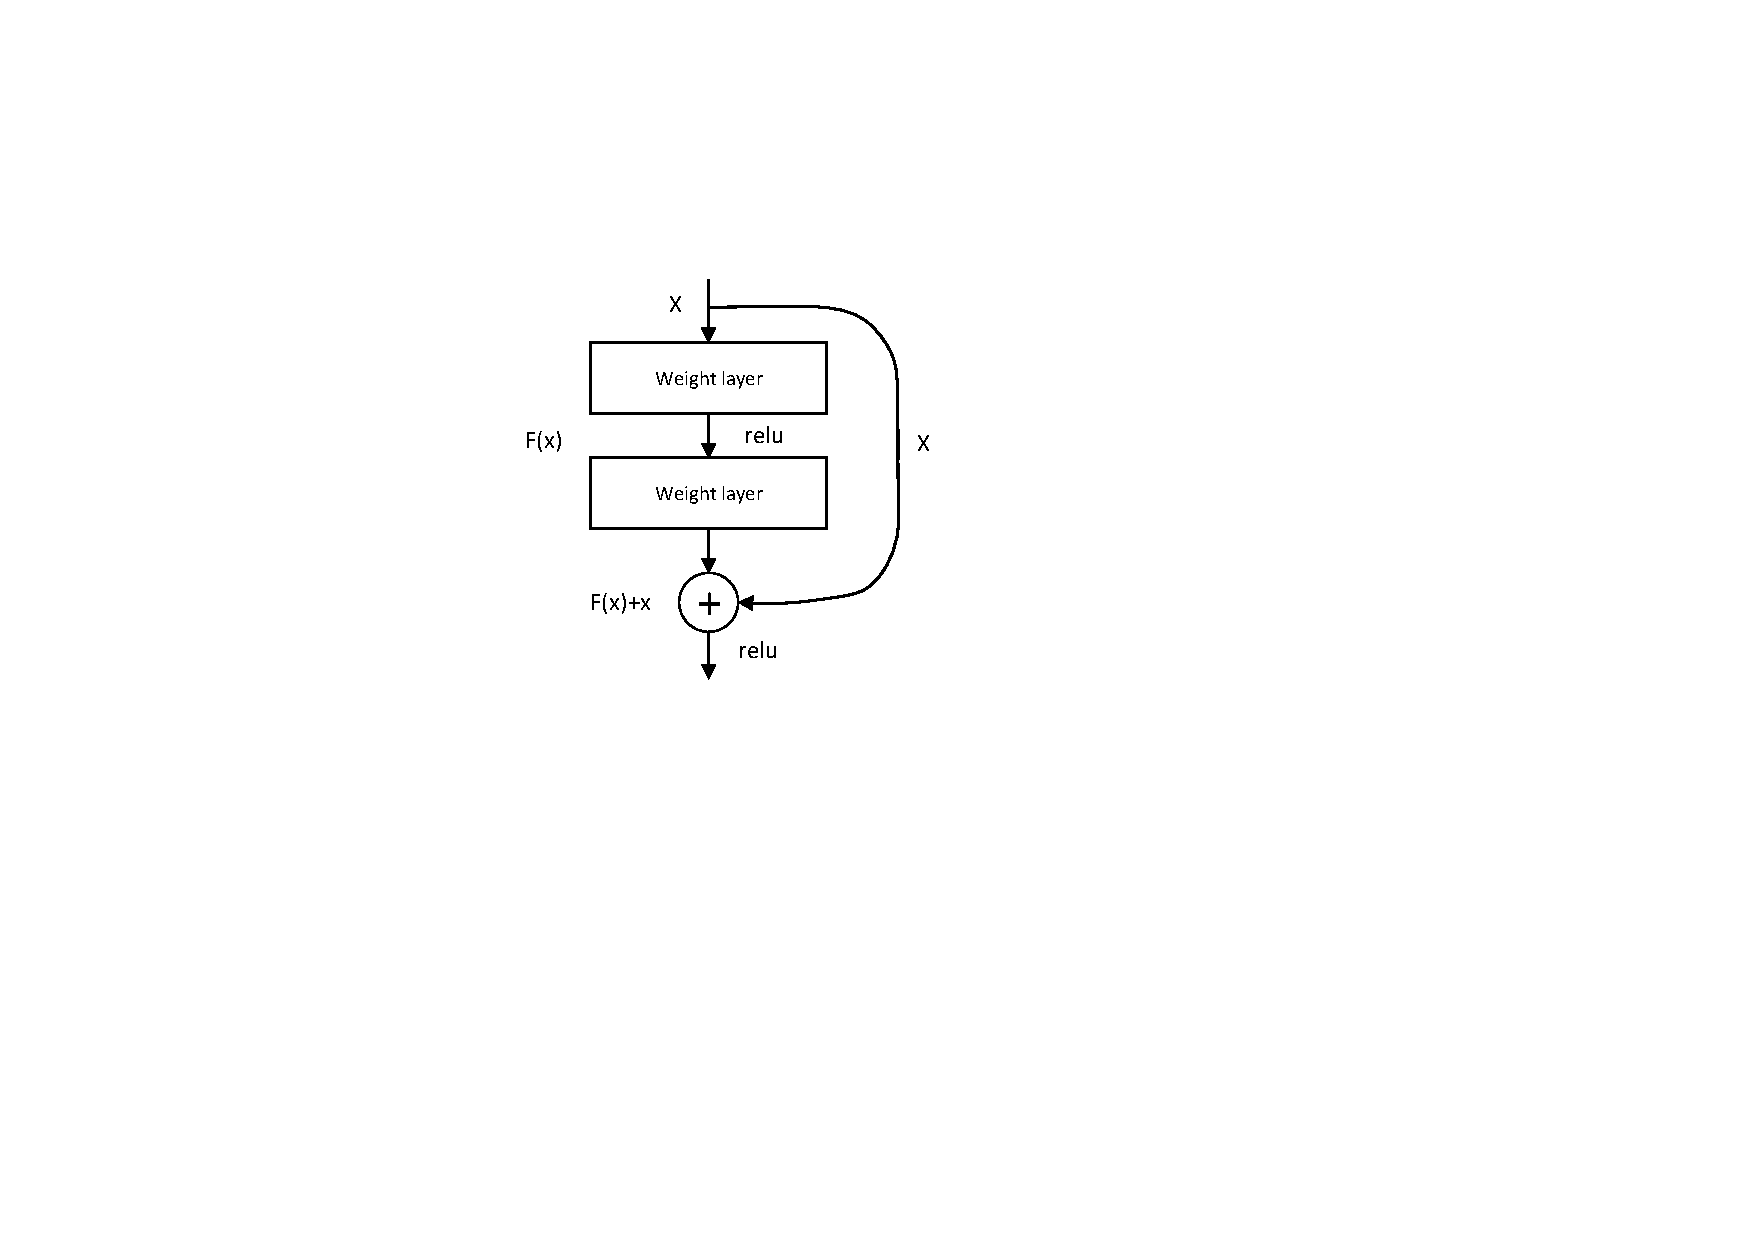
\includegraphics[height=6cm]{residual.pdf}
\caption{残差连接结构图}
\label{residual}
\end{figure}

\textbf{层次归一化Layer normalization}

为了使得模型训练的时候更加容易收敛,减少训练时间,在深度神经网络的模型中加入归一化操作是一个比较常见的做法。在训练卷积神经网络时候,常见的操作是加入批量归一化(Batch Normalization)\upcite{Ioffe:2015:BNA:3045118.3045167},批量归一化通过计算均值和方差将一个批量的输入数据装换到$[0,1]$之间,加速梯度下降,但其高度依赖批量的大小,同时也不适用于输入序列长度不固定的循环神经网络等模型。层次归一化(Layer Normalization)\upcite{ba2016layer}则不是在样本层面,而是将该层神经元的输入通过计算均值和方差转换到在$[0,1]$之间,这样的操作是跨特征计算的,与其他样本无关,因此可以使用任意大小的批量大小。
\begin{align}
	LN(x_i)=\alpha\times\frac{x_i-u_B}{\sqrt{\sigma_B^2+\epsilon}}+\beta
\end{align}
\textbf{Dropout}

使用神经网络时,随着模型变得更大和更深,也带了过拟合的潜在风险,对于神经网络来说,除了在损失函数处加上L1和L2正则项之外,在模型的结构当中加入Dropout也是防止过拟合的常见操作之一,为了防止我们的模型过拟合、同时为了让训练更稳定,减少部分模型参数加速训练过程,在Self-Attention模块的输出之后加上Dropout操作:
\begin{align}
	\hat{y}=x+\text { Dropout }(\text {SA}(\text { LN }(x)))
\end{align}
\textbf{模型训练}

最终模型根据输出序列是否为用户实际点击行为经过$Sigmoid(\cdot )$函数映射到$[0,1]$之间的概率,因此模型的优化目标为最小化如下的交叉熵损失函数:
\begin{align}
-\sum_{{u} \in \mathbb{U}} \sum_{t \in[1,2, \ldots, n]}\left[\log (\hat{y})+\sum_{\hat{s}_{u}^{t}\neq s_{u}^{t}} \log (1-\hat{y})\right]
\end{align}


\section{复杂度分析}

模型的时间复杂度只要由Self-Attention模块主导,Self-Attention的时间复杂度为$O(n^{2} d)$,其中$n$为序列的长度,$d$为嵌入层维度,而Multi-Head Attention由多个Self-Attention并行叠加,假设有$h$个Self-Attention,则Multi-Head Attention的时间复杂度仍为$O(n^{2} d)$,


% \subsection{算法描述}


\section{算法实现}
\begin{algorithm}[H]
	\caption{基于自注意力机制的序列感知推荐算法}
	\label{alg:self-attention}
		\begin{algorithmic}[1]
			\REQUIRE 用户序列数据:$S$;最大序列长度:$maxLen$; 最大字数:$maxNum$
			\ENSURE 推荐结果列表:$Items$
			\STATE $sequences \leftarrow S$, 其中$sequences=\{sen_{1}, sen_{2}...sen_{n}\}$ 
			\FOR {$sequence$ in $input\_sequences$}
			    \STATE $embedding\_sequence()$
			    \STATE $pos\_embedding\_sequence()$
				    \FOR {$Self\_Attention$ in $Multi\_Head\_Attention$}
					    \STATE do $Self\_Attention$()
					    \STATE do $Layer\_Normalize$()
					    \STATE do $FeedForward$()
					    \STATE $input\_sequence$ = $sequence$*Mask
					\ENDFOR
			\ENDFOR
			\FOR {$sequence$ in $output\_sequences$}
			    \STATE $embedding\_sequence()$
			    \STATE $pos\_embedding\_sequence()$
				    \FOR {$Self\_Attention$ in $Multi\_Head\_Attention$}
					    \STATE do $Self\_Attention$()
					    \STATE do $Layer\_Normalize$()
					    \STATE do $FeedForward$()
					    \STATE $output\_sequence$ = $sequence$*Mask
					\ENDFOR
			\ENDFOR
			\STATE $sequence$ = $output_sequence$ + $input_sequence$
			\STATE do $Layer\_Normalize$()
			\FOR {$Self\_Attention$ in $Multi\_Head\_Attention$}
			    \STATE do $Self\_Attention$($sequence$)
			    \STATE do $Layer\_Normalize$($sequence$)
			    \STATE do $FeedForward$($sequence$)
			\ENDFOR
			\STATE $output$ = $Sigmoid(sequence)$
			\STATE $NextItem = Max(output) $
			\RETURN $NextItem$
		\end{algorithmic}
\end{algorithm}


\section{本章小结}

本章节主要针对基于(双向)循环神经网络的序列感知推荐算法难以并行训练的缺点,采用自注意力机制,更进一步提升序列感知推荐算法的性能
介绍本文提出的另外一个基于自注意力机制的序列感知推荐算法,其虽然抛弃了循环神经网络的递归结构,但引入位置信息编码的方式仍然能够捕获到序列位置的变化情况,没有了递归的结构依赖,也使得该模型的训练更容易并行化实现,在不损失推荐结果排序准确性的情况下还能获得较高的性能。


%!TEX root = ../document.tex
\chapter{实验结果与分析}

\section{数据集介绍}

为了比较上文提出的两个算法模型,分别从推荐结果的准确性、和算法训练与结果查询返回效率两个方面分别进行了两组实验。%
因此需要设计两组实验分别从算法推荐准确性和性能两个方面进行验证。本文评估上述两个算法在两个来自真实%
应用上的数据集,这些数据集都包涵用户与物品产生交互的时间戳:

\textbf{MovieLens}:MovieLens\footnote{\url{https://grouplens.org/datasets/movielens/}}是%
用来对推荐模型进行评估的最流行的基准数据集,它是由GroupLens研究组织从MovieLens网站收集的关于用户%
对电影评分的数据集,其中主要的评分文件以“用户ID | 电影ID | 评分 | 时间戳”为一行的格式%
保存了某个用户在某时刻对某个电影做出的评分标准,按照数据量的大小不同,本文选用的MovieLens数据集是%
Movielens-1M。

\textbf{Yoochoose}:Yoochoose\footnote{\url{http://2015.recsyschallenge.com}}数据集是%
2015年推荐系统顶级会议RecSys举办的挑战赛RecSys Challenge 2015上公开使用的目标数据集。%
Yoochoose包含了一个在线电子商务网站在6个月时间内用户所有的点击会话流和购买会话流。这里我只使用了%
点击会话流数据集“yoochoose-clicks.dat”,其中每一行包含了一个点击交互行为,总共有33003944行,%
这里我们抽取了其中的前100万行进行建模实验。%
\begin{table}[]
  \centering
  \caption{序列数据集对比}
  \label{tab:datatable}
    \begin{tabular}{@{}lllllll@{}}
    \toprule
    数据集名称    & 物品数目 & 序列数目 & 交互行为数目 & 平均序列长度  \\ \midrule
    MovieLens-1M & 3706     & 6040 & 1000000 & 165.56 \\
    Yoochoose    & 20843 & 254619 & 1000000 & 3.93 \\ \bottomrule
    \end{tabular}
\end{table}
对于每一种数据集,在特征工程处理部分,需要将其处理成按时间排列的序列,因此需要将交互行为按照时间戳进行预排序,%
将排序好的交互行为按照其所属用户或会话流分组构成序列集合。图\ref{fig:feature_engine}为以Movielens-1M数据集%
为例,特征工程前后数据结构示意图,Yoochoose数据集特征工程与此相同。
不同的算法使用的数据集划分策略不同,下文针对每种算法将详细描述数据集划分策略。具体实验数据明细如表格\ref{tab:datatable}所示。
\begin{figure}[!htb]
   \begin{minipage}{0.48\textwidth}
     \centering
     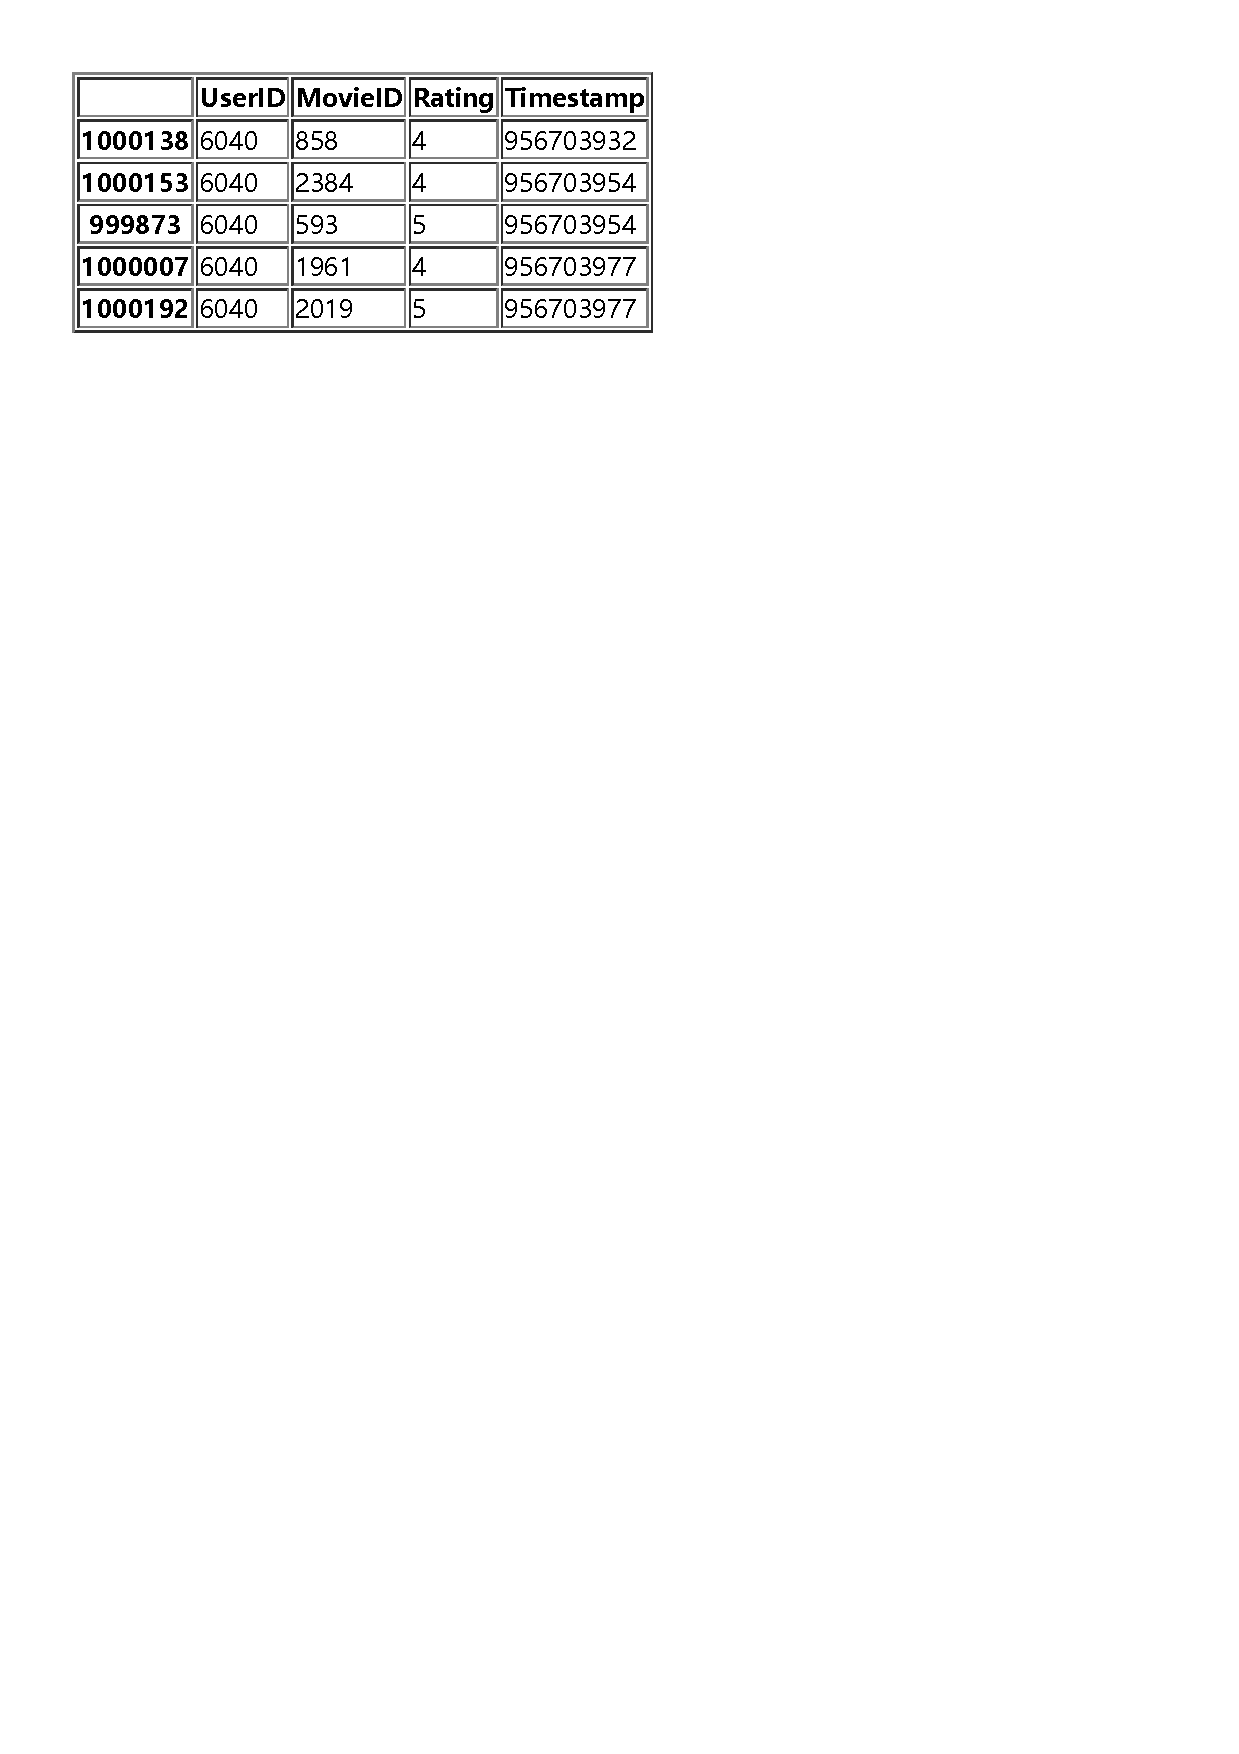
\includegraphics[height=3cm]{MLtable.pdf} % ,width=\linewidth
     \caption{原始数据}
     % \label{Fig:MLtable}
   \end{minipage}\hfill
   \begin {minipage}{0.48\textwidth}
     \centering
     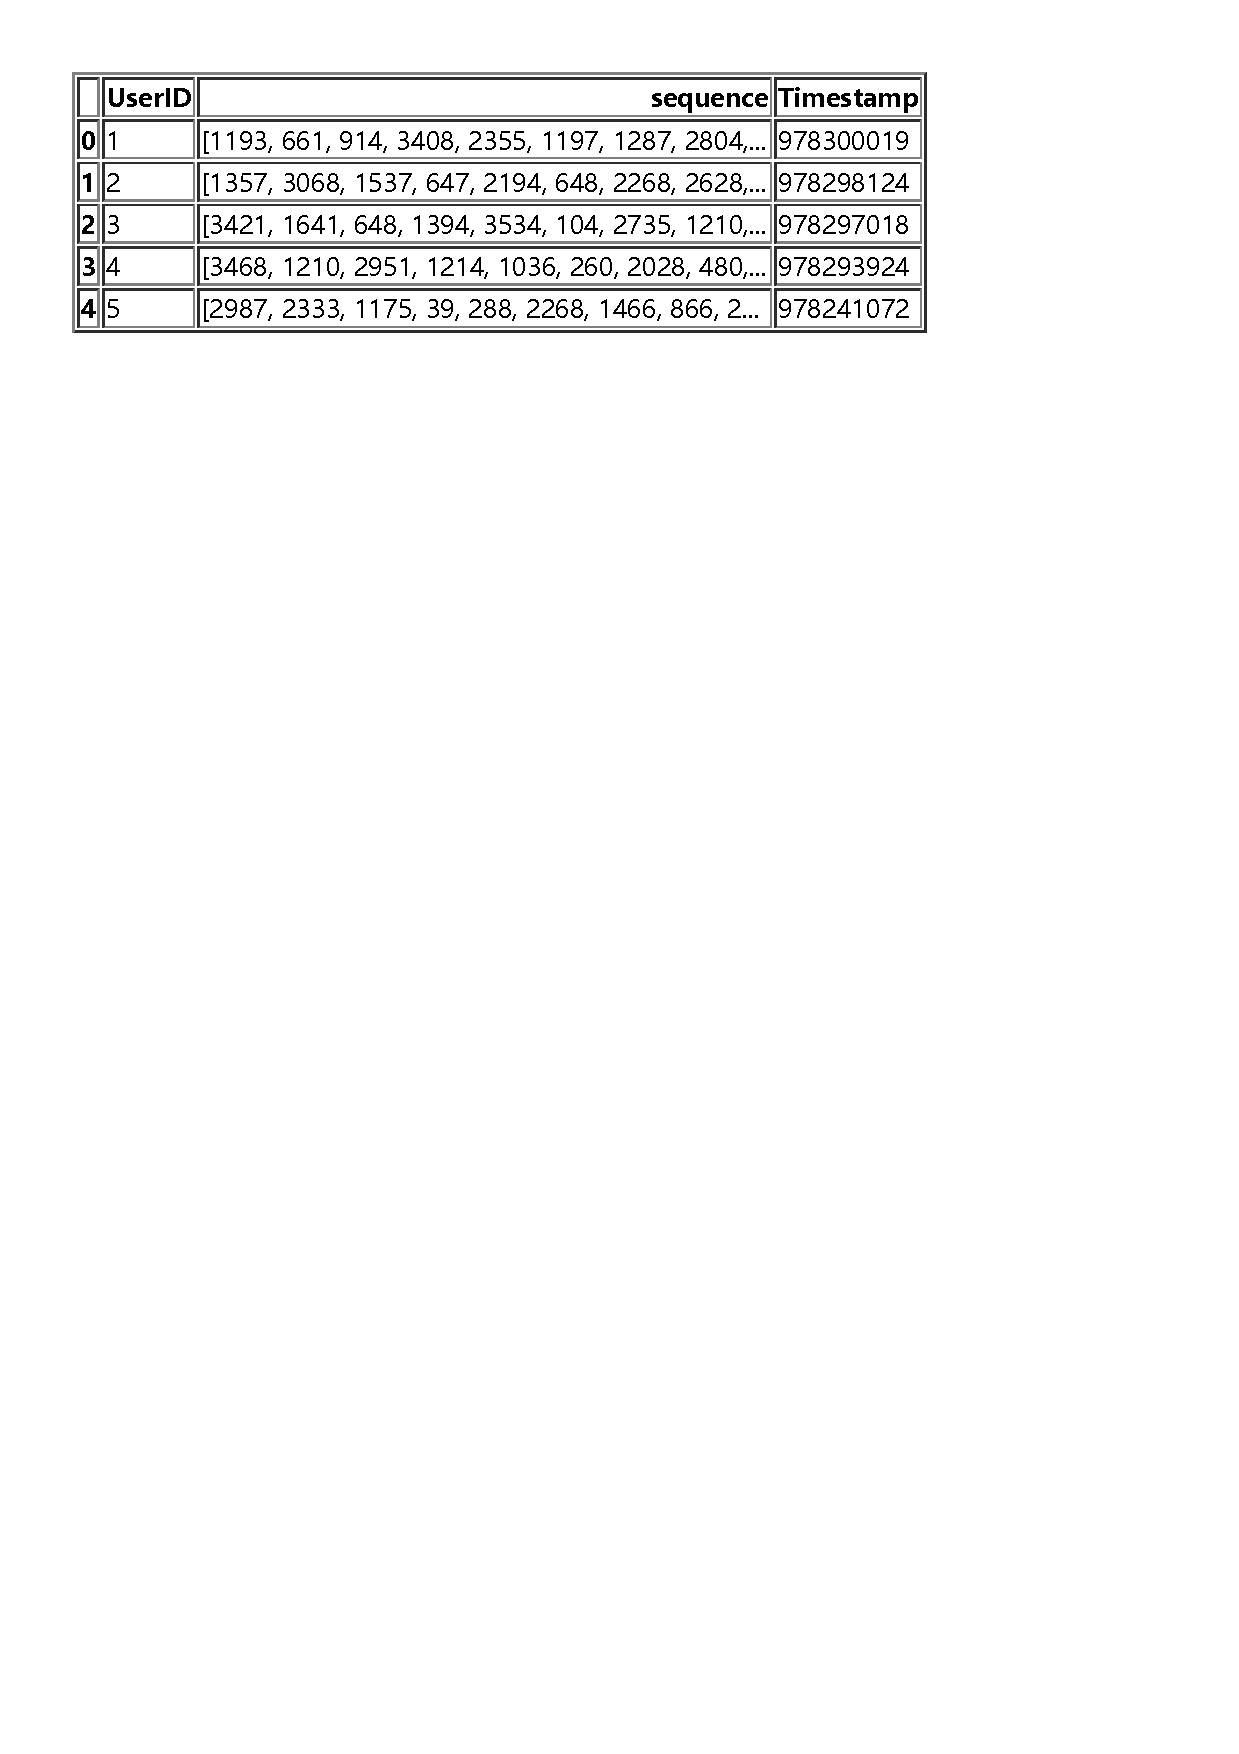
\includegraphics[height=3cm]{MLsequence.pdf} % ,width=\linewidth
     \caption{特征工程处理后数据}
     % \label{Fig:MLsequence}
   \end{minipage}
   \caption{以Movielens-1M数据集为例,将原始交互数据按时间戳排序后分组构成行为序列}
   \label{fig:feature_engine}
\end{figure}


\section{评价指标}
作为一个推荐模型,模型会对查询目标给出点击可能性最高的N个物品,对于本文提出的序列推荐形式,%
模型的输入是$t$时刻及其以前的用户点击物品序列,需要的模型输出目标是$t+1$时刻用户可能点击%
的物品,以$\hat{I}_{u}^{t+1}$表示,所以本文采用了$Precision@N$, $Recall@N$指标来评估%
我们的模型,其计算形式如下:
\begin{equation}
Precision@N=\frac{\sum_{u}|\hat{I}_{u}^{t+1}\cap I_{u}^{t+1} |}{\left | \mathbb{U} \right |*N}
\end{equation}
\begin{equation}
Recall@N=\frac{\sum_{u}|\hat{I}_{u}^{t+1}\cap I_{u}^{t+1} |}{\left |\sum_{u}|I_{u}^{t+1}| \right |}
\end{equation}
由于$Precision@N$和$Recall@N$值可以通过阈值调整来相互权衡,为了得到一个更加容易量化评估%
的指标,本文引入了$F1@N$指标,如果$F1@N$分数越大,可以认为模型的效果更好。而当一次为%
用户推荐多个结果时,推荐结果在屏幕上展示的位置也会影响物品被点击的概率,越靠前的物品越可能被点击,%
约强相关的推荐物品应该出现在结果列表的越前面,而引入$NDCG@N$\upcite{NIPS2009_3758}指标的原因就是为了感知这种%
位置的影响,让点击率越高的物品位置越靠前,$NDCG@N$%
值越接近1,得到的相关推荐结果中前N个物品的排序越准确,所以$F1@N$和$NDCG@N$的计算形式如下:
\begin{equation}
F1@N=\frac{2\times Precision@N\times Recall@N}{Precision@N+Recall@N}
\end{equation}
\begin{equation}
  \begin{aligned}
  DCG@N &= \sum_{i=1}^{N} \frac{2^{rel_{i}}-1}{\log _{2}(i+1)} \\
  IDCG@N &= \sum_{i=1}^{|REL|} \frac{2^{rel_{i}}-1}{\log _{2}(i+1)} \\
  NDCG@N &= \frac{DCG@N}{IDCG@N}
  \label{E21}
  \end{aligned}
\end{equation}
当推荐的物品是用户点击的内容时$DCG@N$中$rel$取值为1,否则$rel$取值为0。而由于每条样本仅有一条为相关,其余均为不相关,所以 $IDCG@N$ 对于每条样本都是一样的,即$\frac{1}{\log 2}$。

\section{实验环境}
\begin{table}[H]
\centering
\caption{实验软硬件环境配置表}
\label{tab:set}
  \begin{tabular}{@{}ll@{}}
  \toprule
  实验环境 & 环境配置                                  \\ \midrule
  CPU  & Intel(R) Xeon(R) CPU E5-2650 v3 @ 2.30GHz *2 \\
  GPU  & Tesla K80 *4                                 \\
  内存   & 64126MB                                      \\
  OS   & CentOS Linux 7 (Core)                        \\
  编程语言 & Python 3.6.8                                 \\
  开发工具 & TensorFlow-GPU 1.12.0                        \\ \bottomrule
  \end{tabular}
\end{table}

\section{基于双向LSTM的序列感知算法实验过程}

本节将通过实验来验证第三章中提出的基于双向LSTM的序列感知算法的有效性,主要介绍针对该实验的数据集处理策略、实验主要研究的问题、影响结果的主要因素。
基于双向LSTM的序列感知算法的特征工程部分,首先将每个交互样本按照时间戳从先到后排列,然后根据交互样本所属用户聚类构成行为序列,在序列感知推荐算法当中不需要用户的评分数据因此可以去除。对于行为序列长度小于5的序列进行了过滤,剩余序列集合前80\%划分为训练集,后20\%划分为测试集。将序列中最后一个交互物品ID作为模型学习的标签,截取序列中最近的$N$个物品作为BiLSTM的输入序列,其中$N\geq 1$,当$N>1$而存在序列的长度不足时,在长度不足序列的前部进行特殊值填充以表示缺失。当时间窗口为1时,意味着我们将序列的最后一个物品作为标签,最近的一个物品作为序列的特征输入模型就行学习。

BiLSTM模型的实现基于开源深度学习框架Keras,以Tensorflow作为其后端。使用批量梯度下降法Adam作为优化器,并设置初始学习率$\alpha$为0.01,学习率衰减权重因子$\beta$为0.9。其他超参数本实验首先使用常见值作为初始值,为了得到更好的性能,使用网格搜索的形式自动寻找最优参数组合,但这会带来极大的计算量。经过多次尝试,本实验最终选定了以下超参数组合:嵌入层因子$|e|=100$,循环层神经元数目$H=200$,全连接层神经元数目$O=100$,梯度下降批量大小为32。在训练阶段为避免过拟合,当验证数据上经过3个batch损失函数仍没有下降则EarlyStopping。

为了探求基于双向LSTM的序列感知算法需要的序列长度,将超参数固定之后本文也设置了对比实验探求不同序列长度对模型的影响,图\ref{fig:windows}显示了在MovieLens-1M数据集上输入序列长度分别从1\~10时,训练阶段EarlyStopping时最优的损失函数值。
\begin{figure}[htb]%更改
  \centering
  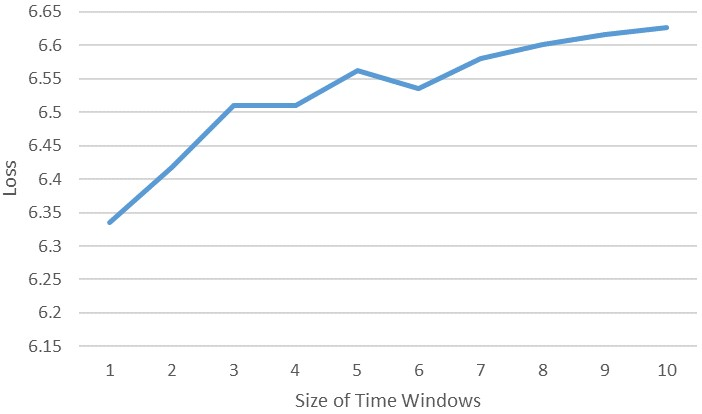
\includegraphics[width=12cm]{Loss_timewindows.jpg}
  \caption{BiLSTM在MovieLens-1M数据上不同序列长度的最小训练loss}
  \label{fig:windows}
\end{figure}
通过图\ref{fig:windows}中可以看到,在不同的输入序列长度下,BiLSTM的性能有稍微为降低,为了模型的稳定性选取了中位值5作为最终序列长度。
图\ref{fig:BiLSTMloss}显示了固定时间窗口为5及其他超参数的情况下,训练集和测试集上的损失函数下降图。
\begin{figure}[htb]%更改
  \centering
  \includegraphics[width=12cm]{model_loss-eps-converted-to.pdf}
  \caption{BiLSTM在MovieLens-1M数据上不同序列长度的最小训练loss}
  \label{fig:BiLSTMloss}
\end{figure}

\section{基于自注意力机制的序列感知算法实验过程}
本节将通过实验来验证第四章中提出的基于自注意力机制的序列感知算法的有效性。
与基于双向LSTM的序列感知算法的特征工程部分一样,首先将每个交互样本按照时间戳从先到后排列,然后根据交互样本所属用户聚类构成行为序列。
在数据集划分部分,由于基于自注意力机制的序列感知算法包含Encoder-Decoder结构,Decoder对应的输出序列由输入序列往后滑动一个窗口构成,
在数据集划分部分也使用了同样的划分策略,将所有序列截止倒数第三个位置之前部分划分为训练集,截止倒数第二个之前部分划分为验证集,包含最后一个物品的序列作为测试集,超过最大长度$N$部分做截取处理。

图\ref{fig:Slefattentionloss}为学习率分别设置为0.001、0.003、0.01时训练集上的损失函数的下降曲线,从图中可以看到,
Transformer4Rec模型在MovieLens-1M上使用合适的学习率损失函数可以更快收敛,节省训练时间,因此后文实验以学习率0.01为基础进行。
\begin{figure}[htb]%更改
  \centering
  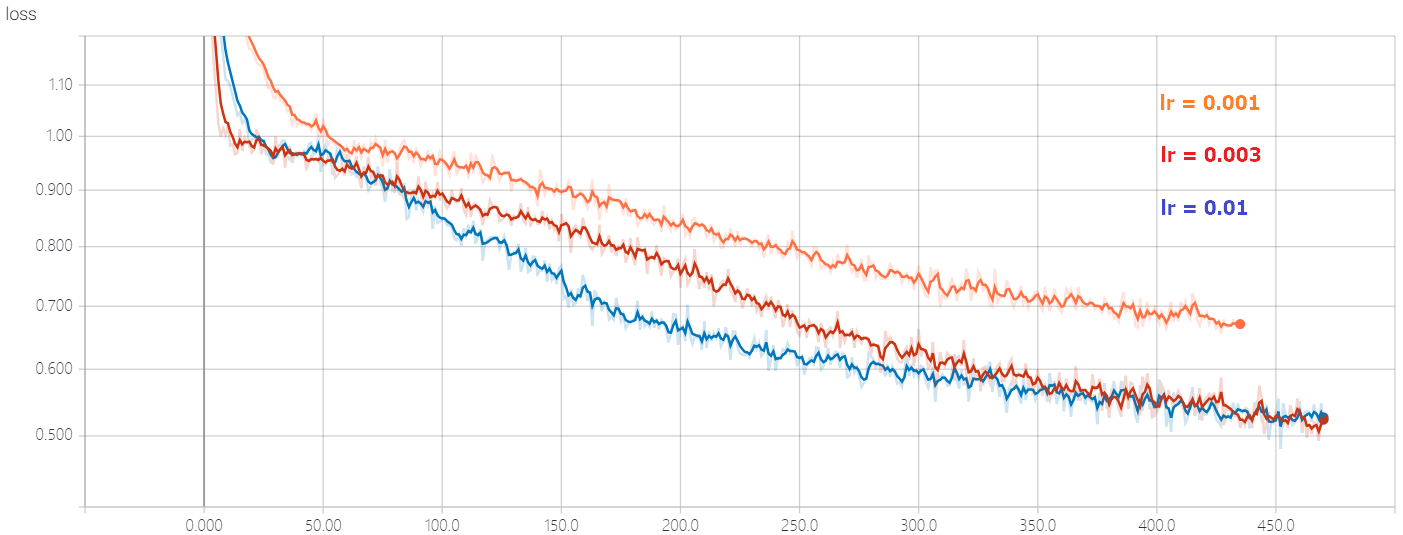
\includegraphics[width=12cm]{2019-03-31-174902.png}
  \caption{Transformer4Rec在MovieLens-1M数据上学习率分别设置为0.001、0.003、0.01时训练集上的损失函数的下降曲线}
  \label{fig:Slefattentionloss}
\end{figure}

模型输入序列的长度也是影响模型性能的关键因素之一,在固定学习率及其他超参数之后本节试验了不同长度序列对模型性能的影响,如图
\ref{fig:maxlenloss}所示,从图中可以看到不同序列长度对模型性能的影响不是非常明显,但越长的序列它的迭代过程越慢,综合考虑
性能与效率的原因,在本节MovieLens-1M数据集上最大序列长度设为150,在Yoochoose数据集上最大长度设为50。
\begin{figure}[htb]%更改
  \centering
  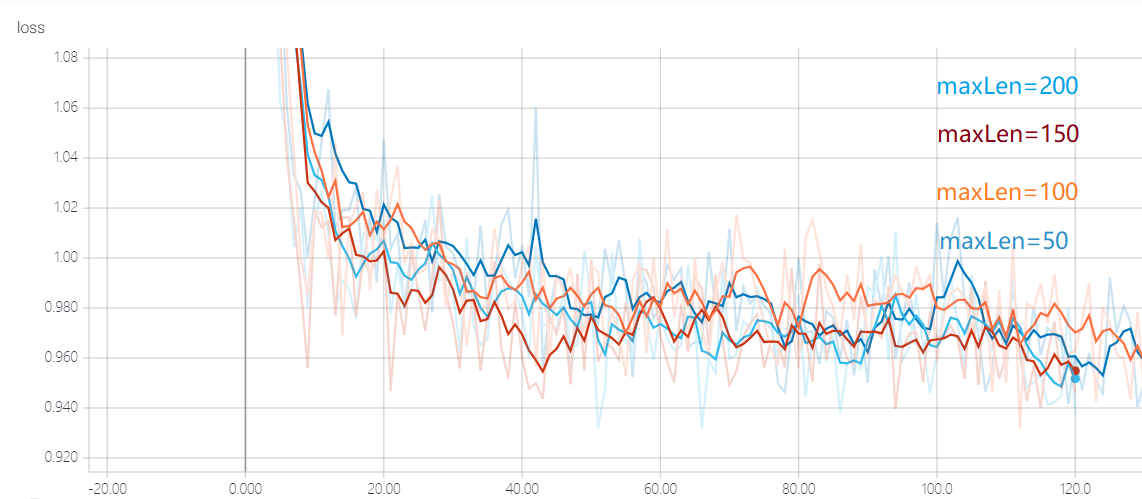
\includegraphics[width=12cm]{2019-03-31-220433.png}
  \caption{Transformer4Rec在MovieLens-1M数据上最大序列长度分别设置为200、150、100、50时训练集上的损失函数的下降曲线}
  \label{fig:maxlenloss}
\end{figure}
其他重要超参数如Dropout比率、Multi-Head Attention中Self-Attention个数、批量大小、迭代次数、隐藏层神经元数目等,经过
自动网格搜索后分别确定为:0.2、2、128、10、50。

% \subsection{实验三}

\subsection{对比实验}
\textbf{POP}:最流行物品推荐法POP作为本文选择的最简单的基准线,通过统计训练数据中出现次数最多的物品,推荐策略为为用户推荐那些他还没有看过的最热门的物品。

\textbf{GRU4Rec\upcite{DBLP:journals/corr/HidasiKBT15,Hidasi:2018:RNN:3269206.3271761}}:GRU4Rec是序列感知推荐领域最重要的算法之一,2016年Balazs Hidasi等人首次将循环神经网络的方法应用到基于会话的个性化推荐领域,并取得了当时的最好效果,因此本文将其作为\textit{基于循环神经网络的序列感知推荐算法}中的代表,其代码基于Keras\upcite{chollet2015keras}提供的GRU高层API实现。

\textbf{Caser\upcite{Tang:2018:PTS:3159652.3159656}}:2018年Jiaxi Tang等人将序列嵌入矩阵使用CNN提取特征,提出了卷积序列嵌入推荐模型Caser,因此本文将其作为\textit{基于卷积神经网络的序列感知推荐算法}中的代表,其代码实现基于原作者开源的PyTorch实现版本\upcite{paszke2017automatic}。

本文讨论的两个模型与三个对比模型的分别在MovieLens-1M与Yoochoose数据集上的实验结果如表\ref{table:result}所示。使用双向长短期记忆网络的BiLSTM4Rec模型相比GRU4Rec,有约15\%的推荐准确性提升。

% Please add the following required packages to your document preamble:
% \usepackage{booktabs}
% \usepackage{multirow}
\begin{table}[]
\centering
\caption{各算法评价指标结果}
\label{table:result}
  \begin{tabular}{@{}lllllll@{}}
  \toprule
  数据集名称                     & 测评指标      & POP      & GRU4Rec  & \textbf{BiLSTM} & Caser & \textbf{Self-Attention} \\ \midrule
  \multirow{4}{*}{MovieLens-1M} & Recall@10    & 0.041390 & 0.109286 & 0.125679 & 0.1344 & 0.7055      \\
                                & Precision@10 & 0.004139 & 0.010928 & 0.012567 & 0.0112 & 0.0705      \\
                                & F1@10        & 0.007526 & 0.019870 & 0.023052 & 0.0244 & 0.1279      \\
                                & NDCG@10      & 0.019398 & 0.056077 & 0.064489 & 0.4538 & 0.4398      \\
  \multirow{4}{*}{Yoochoose}    & Recall@10    & 0.041493 & 0.105735 & 0.121595 & 0.1374 & 0.8134      \\
                                & Precision@10 & 0.004149 & 0.010573 & 0.012159 & 0.0137 & 0.0813      \\
                                & F1@10        & 0.007544 & 0.019224 & 0.022107 & 0.0249 & 0.1483      \\
                                & NDCG@10      & 0.019779 & 0.055170 & 0.063445 & 0.4621 & 0.5066      \\ \cmidrule(l){2-7} 
  \end{tabular}
\end{table}

% \section{实验结果与分析}



% \subsection{结果分析}

\section{算法运行时间比较}

在3.4节和4.3节,分别分析了第三章基于双向LSTM的序列感知推荐方法和第四章基于自注意力机制的%
序列感知推荐方法的时间复杂度,表\ref{tab:runtime}给出了本实验中各个算法在测试集上预测的运行时间,%
其中MovieLens-1M测试集中包含1208条平均序列长度为165.56的样本,由于对序列长度小于5的用户数据进行了过滤,Yoochoose测试集中包含43298条平均长度为10.09的样本,
对于每个样本,每种算法都给出可能性
最高的10个推荐结果,测试集算法运行时间不包含评估阶段。
\begin{table}[]
\centering
\caption{各算法测试集预测时间比较}
\label{tab:runtime}
\begin{tabular}{@{}llllll@{}}
数据集          & POP  & GRU4Rec & Caser & BiLSTM & Self-Attention \\ \midrule
Movielens-1M & 1.99ms &  18.35s  & 19.1s &  21.1s   &    1.7s         \\ \bottomrule
Yoochoose    & 17.5ms &  30.7s   & 31.98s &  46.9s  &    11.3s      
\end{tabular}
\end{table}
基于双向循环神经网络的BiLSTM方法正向与反向可以并行,基于卷积结构的Caser算法在进行序列建模时,长序列的记忆能力严重依赖网络的深度,

\section{本章小结}




%!TEX root = ../document.tex
\chapter{总结与展望}
\label{chap:conclusion}

\section{论文总结}
推荐系统是数据挖掘与机器学习领域中最成功的应用之一,推荐算法作为推荐系统的灵魂,支撑着系统的表现。经典推荐算法面对大数据的压力时往往显得力不从心,而基于梯度下降优化的深度学习推荐算法没有理论上大数据上限。现有的推荐算法又往往忽视了隐藏在用户行为之中的时序关系,目前大多数深度学习推荐算法又需要大量的特征,当面对缺少用户隐私数据的场景这些算法都将无能为力。为了应对当前推荐算法这几个方面面临的问题,本文完成的工作如下:
\begin{enumerate}
    \item 本文调研了深度学习在推荐系统应用领域的发展情况,针对现有推荐算法都需要使用大量用户隐私%
          数据构造特征的情况下,提出了只利用用户历史行为序列的序列感知推荐算法。
    \item 本文设计了基于双向长短期记忆网络的序列感知推荐模型BiLSTM4Rec,对用户历史行为序列进行嵌入式表达,生成稠密矩阵,%
          利用双向长短期记忆网络对嵌入矩阵进行序列建模,预测下一个物品,将推荐问题转变成一个多分类问题。
    \item 考虑到循环神经网络难以并行训练的效率问题,本文抛弃神经网络循环结构,从Transformer\upcite{NIPS2017_7181}
    	  模型中抽取Self-Attention模块,%
          提出Transformer4Rec模型,该模型在获得较大%
          推荐精度的情况下还不损失性能。
\end{enumerate}

\section{论文展望}

本文主要针对序列感知推荐领域进行了研究,利用神经网络序列建模技术,有效的提高了推荐结果的精确性,取得了一定的工作成果。但是序列感知推荐领域还存在许多的难题,这也是我们未来工作中可以持续改进的部分,主要包括以下几点:
\begin{enumerate}
    \item 本文提出的两个序列感知推荐算法主要利用了深度学习中的序列建模技术,但深度学习模型的可解释性很差,而推荐系统中又存在大量的需要可解释性场景,在后期的研究中,应使用具有可解释性的序列建模技术,例如图神经网络。
    \item 本文提出的序列感知推荐方法不需要大量的用户隐私数据与物品属性特征,但为了虽然满足某些特定的应用场景,但为了获得具有更加鲁棒性的推荐模型,应考虑将序列感知模型与现有的推荐模型结合,让不同特点的模型发挥各自的优点。
    \item 本文对基于神经网络的序列感知模型进行了粗略的设计与实现,但由于时间与条件的限制,还要许多细节没有完善,与现有的许多成熟推荐模型相比还有相当大的差距,在后期的工作中,将对本模型进行持续完善,使其能成为当今领域推荐算法工具箱中的一员。
\end{enumerate}


% 参考文献
\cleardoublepage
\renewcommand{\chapterlabel}{\bibname} % 设置参考文献的页眉
\bibliographystyle{bstutf8}
\bibliography{ref/refs}



% 附录
%\appendix
%\backmatter
%%%% Local Variables:
%%% mode: latex
%%% TeX-master: "../main"
%%% End:

\chapter{外文资料原文}

%\input{data/appendix02}

%\begin{denotation}

% \item[SCNU] 华南师范大学 (South China Normal University)
%\item[DKA] 学术社交网络(Academic Social Networks)

\item[CF] 协同过滤 (Collaborative Filtering)
\item[UBCF] 基于用户的协同过滤  (User-based Collaborative Filtering,UBCF)
\item[IBCF] 基于物品的协同过滤  (Item-based Collaborative Filtering,IBCF)
\item[RNN] 循环神经网络 (Recurrent Neural Network)
\item[LSTM] 长短期记忆神经网络 (Long Short-Term Memory)
\item[ANN] 人工神经网络 (Artificial Neural Network)
\item[FNN] 前馈神经网络 (Feedforward Neural Network)
\item[MLP] 多层感知机 (Multi-Layer Perceptron)
\item[BRNN] 双向循环神经网络 (Bi-directional Recurrent Neural Network)
\item[GRU] 门控循环单元 (Gated Recurrent Unit)
%\item[cluster] 集群
%\item[graphic] 图形
%\item[communication] 通信
%\item[3D] 三维 (Three Dimemsion)
%\item[BMP] 位图
%\item[PNG] 便携式网络图形 (Portable Network Graphics)
%\item[Watershed] 分水岭
%\item[GUI] 图形用户界面 (Graphical User Interface)
%\item[$E$] 能量
%\item[$m$] 质量
%\item[$c$] 光速
%\item[$P$] 概率
%\item[$T$] 时间
%\item[$v$] 速度

\end{denotation}
 % 如果要生成符号列表
\listoftables           % 如果要生成表目录
\listoffigures          % 如果要生成图目录

% 致谢
\cleardoublepage
\renewcommand{\chapterlabel}{\ackname} % 设置参考文献的页眉
\begin{ack}
光阴似箭,日月如棱,三年的时间,我的硕士生涯已接近尾声,回头想想这段短暂的求学路,时而喜悦,时而惆怅,感谢命运的安排,让我有幸结识了许多良师益友。首先感谢我的恩师朱佳教授,谢谢您一直以来对我的照顾,让我有幸遇到您这样对学生亦师亦友的好导师,您和蔼可亲、学识渊博、没有架子以及乐观向上的工作生活态度深深感染着我。感谢您耐心指导我的论文工作,感谢您陪我走过人生最重要的结婚典礼,感谢您带领我们参加各种会议开阔视野,感谢您带我们吃各种美食,感谢您跟我们聊各种八卦新闻。。。再次向您致以衷心的感谢和崇高的敬意。

感谢学者网团队的各位小伙伴,肖丹阳、林雪琴、韦经敏,感谢你们的3年陪伴和对我的学术帮助,感谢332实验室的师弟师妹们,杨芬、汪序明、郑泽涛、伦家琪、胡迎彬、于晗宇,感谢你们带给我的欢乐和帮助,感谢已经毕业的师兄师姐,董浩业、丁蕊、陈凌潇、许传华、孔剑龙,跟你们在一起真的很开心快乐,感谢生活学习中有你们。

感谢我的最佳室友们男神玉、波波、嘉良,跟你们在一起的日子真的很幸福,记得大半夜去外面吃烧烤喝啤酒,记得去自助KTV嗨翻全场,记得在宿舍吃着零食聊学术八卦到深夜,这些美好的时光将是我一生宝贵的财富,谢谢你们的陪伴,让我的研究生生活丰富多彩。

感谢我的父母、岳父母、爱人、女儿及所有的亲朋好友,你们是我永远的支持者,让我在学习和生活中都受到你们的无私关怀和帮助,才能完成研究生求学生涯,感谢你们的付出,让我开心的度过每一天。

感谢所有的2016级的同窗们,谢谢你们陪我一起成长,祝各位同窗前程似锦;感谢我的母校华南师范大学,谢谢您为我们提供美好的校园环境和学习氛围,祝您的办学越来越好;最后感谢各位答辩评委老师,谢谢你们为我指点出不足,祝各位老师永远健康快乐。

\end{ack}


% 作者攻读学位期间发表的学术论文目录
\cleardoublepage
\renewcommand{\chapterlabel}{\resumename} % 设置作者个人成果的页眉
\begin{resume}

  \section*{发表的学术论文} % 发表的和录用的合在一起

  \begin{enumerate}[{[}1{]}]
  \addtolength{\itemsep}{-.36\baselineskip}%缩小条目之间的间距,下面类似
  \item Hailin F, Jianguo L, Jiemin C, et al. Sequence-based Recommendation with Bidirectional LSTM Network[C]. PCM 2018: 428--438.(第一作者)
  \item Jiemin C, Jianguo L, Jing X, et al. A Hybrid Collaborative Filtering Model: RSVD Meets Weighted-Network Based Inference[J]. 網際網路技術學刊 2016: 1221-1233.(合作作者)  
  \end{enumerate}

  % \section*{研究成果} % 有就写,没有就删除
  % \begin{enumerate}[{[}1{]}]
  % \addtolength{\itemsep}{-.36\baselineskip}%
 
  % \item 基于海量文献数据挖掘研究热点和推荐学者的系统1.0.软件著作权(2017SR380708).(第一作者)
  % \item 基于微博数据的电影分析系统统1.0.软件著作权(2017SR384142).(第一作者)
  % \item 基于互联网信息的房产分析系统统1.0.软件著作权(2017SR380714).(合作作者)
  % \item 面向空气质量的网络爬虫系统统1.0.软件著作权(2018SR168761).(合作作者)
  % \item 一种基于深度学习的医疗记录模型构建方法、系统及装置统1.0.中国专利(201711247467.6).(合作作者)
  % \end{enumerate}
\end{resume}


\end{document}
%%
